\documentclass[xcolor={dvipsnames},aspectratio=169,10pt]{beamer}

% chktex-file 41

% check for obsoleted LaTeX packages
\usepackage[l2tabu,orthodox]{nag}

% utility packages
\usepackage{etoolbox}
\usepackage{xifthen}
\usepackage{xpatch}
\usepackage{adjustbox}

% better text justifying
\usepackage{microtype}
% justify text inside list environment
% Ref: http://liam0205.me/2017/04/11/justifying-in-beamer-s-lists/
\usepackage{ragged2e}
\makeatletter
\xpatchcmd{\itemize}{\raggedright}{\justifying}{}{}
\xpatchcmd{\beamer@enum@}{\raggedright}{\justifying}{}{}
\xpatchcmd{\@@description}{\raggedright}{\justifying}{}{}
\makeatother

% math related packages
\usepackage{amsmath}
\usepackage{amssymb}
\let\emptyset\varnothing%
\usepackage{amsfonts}
\usepackage{mathrsfs}
\usepackage{latexsym}
\usepackage{bm}
\usepackage{fancynum}

% equation style
\newcommand{\setdisplayskip}{%
  \abovedisplayskip=0.25\baselineskip plus 0.05\baselineskip minus 0.125\baselineskip% chktex 1
  \abovedisplayshortskip=0pt plus 0.075\baselineskip% chktex 1
  \belowdisplayskip=0.25\baselineskip plus 0.05\baselineskip minus 0.125\baselineskip% chktex 1
  \belowdisplayshortskip=0.15\baselineskip plus 0.075\baselineskip minus 0.075\baselineskip% chktex 1
}
\apptocmd\Huge{\setdisplayskip}{}{}
\apptocmd\huge{\setdisplayskip}{}{}
\apptocmd\LARGE{\setdisplayskip}{}{}
\apptocmd\Large{\setdisplayskip}{}{}
\apptocmd\large{\setdisplayskip}{}{}
\apptocmd\normalsize{\setdisplayskip}{}{}
\apptocmd\small{\setdisplayskip}{}{}
\apptocmd\footnotesize{\setdisplayskip}{}{}
\apptocmd\scriptsize{\setdisplayskip}{}{}
\apptocmd\tiny{\setdisplayskip}{}{}

% figure related packages
\usepackage{graphicx}
\usepackage{tikz}
\usetikzlibrary{backgrounds,calc,decorations.pathreplacing,fit,matrix,patterns,positioning,shapes,shapes.multipart}
\usepackage{pgfplots}
\pgfplotsset{compat=1.16}
\usepackage[outline]{contour}
\contourlength{1.8pt}
\usepackage{pifont}
\makeatletter
% Ref: https://tex.stackexchange.com/a/62273
\newenvironment{customlegend}[1][]{%
  \begingroup
  \csname pgfplots@init@cleared@structures\endcsname
  \pgfplotsset{#1}
  \def\addlegendimage{\csname pgfplots@addlegendimage\endcsname}
  \def\addlegendentry{\csname pgfplots@addlegendentry\endcsname}
}{%
  \csname pgfplots@createlegend\endcsname
  \endgroup
}%
\makeatother

% table related packages
\usepackage{array}
\usepackage{tabu}
\usepackage{booktabs}
\usepackage{multirow}
\newcommand{\tabincell}[2]{\begin{tabular}{@{}#1@{}}#2\end{tabular}}
\usepackage{threeparttable}
\newcolumntype{C}{>{$}c<{$}}
\newcolumntype{L}{>{$}l<{$}}

% hyperref setting
\hypersetup{
  unicode,
  psdextra,
  bookmarksnumbered=true,
  bookmarksopen=true,
  bookmarksopenlevel=3,
  bookmarksdepth=4,
  pdfcenterwindow=true,
  pdfstartview={Fit},
  pdfpagemode={FullScreen},
  pdfpagelayout={SinglePage},
}
\usepackage{bookmark}

% beamer theme
\usetheme{metropolis}
\metroset{block=fill,numbering=fraction}
\usepackage{appendixnumberbeamer}

% caption style
\setlength\abovecaptionskip{3pt}
\setbeamerfont{caption}{size=\scriptsize}
\renewcommand{\figurename}{Fig.}
\usepackage[font=scriptsize]{subcaption}

% bibliography
\usepackage[
  style=ieee-alphabetic,
  doi=false,
  isbn=false,
  giveninits=true,
  dashed=false,
  maxbibnames=10,
]{biblatex}
\setcounter{biburllcpenalty}{1}
\setcounter{biburlucpenalty}{1}
\setcounter{biburlnumpenalty}{1}

\addbibresource{ref.bib}

\title{Authenticated Query Processing in the Cloud}
\author{XU Cheng}
\institute{Supervisor: Prof.~XU Jianliang}
\date{January 31, 2019}
\titlegraphic{\hfill\resizebox{!}{0.7cm}{\definecolor{c040a82}{RGB}{4,10,130}
\begin{tikzpicture}[y=0.80pt, x=0.80pt, yscale=-1.000000, xscale=1.000000, inner sep=0pt, outer sep=0pt]
  \path[fill=c040a82] (321.9029,153.3392) -- (321.9029,129.8392) --
  (324.4029,129.8392) .. controls (326.2485,129.8392) and (326.9029,130.3706) ..
  (326.9029,131.8692) .. controls (326.9029,133.8717) and (326.9430,133.8694) ..
  (329.8739,131.7025) .. controls (331.9134,130.1947) and (334.2771,129.5059) ..
  (337.4122,129.5059) .. controls (346.0462,129.5059) and (350.8998,135.7433) ..
  (350.8998,146.8392) .. controls (350.8998,154.6277) and (348.8323,159.3444) ..
  (344.0050,162.5693) .. controls (339.7947,165.3820) and (334.4820,165.4897) ..
  (330.1529,162.8502) -- (326.9029,160.8686) -- (326.9029,168.8539) .. controls
  (326.9029,176.7049) and (326.8608,176.8392) .. (324.4029,176.8392) --
  (321.9029,176.8392) -- cycle(342.3140,156.7625) .. controls
  (344.5428,154.1137) and (344.9029,152.7415) .. (344.9029,146.8973) .. controls
  (344.9029,141.6412) and (344.4550,139.5396) .. (342.9187,137.5865) .. controls
  (339.0935,132.7234) and (331.6343,133.2355) .. (328.7866,138.5565) .. controls
  (327.9993,140.0276) and (327.4029,144.0592) .. (327.4029,147.9100) .. controls
  (327.4029,153.6966) and (327.7544,155.0523) .. (329.8272,157.2587) .. controls
  (333.4075,161.0697) and (338.8724,160.8525) .. (342.3140,156.7625) --
  cycle(72.4029,169.1710) .. controls (41.4482,165.3684) and (17.7187,156.1189)
  .. (12.3670,145.7697) .. controls (8.8979,139.0613) and (11.5209,132.2149) ..
  (19.5248,127.0866) .. controls (28.4508,121.3675) and (52.9327,114.8392) ..
  (65.4541,114.8392) .. controls (67.7634,114.8392) and (71.0591,114.5580) ..
  (72.7779,114.2142) -- (75.9029,113.5892) -- (75.9029,89.7595) --
  (75.9029,65.9298) -- (72.6529,65.4007) .. controls (70.8654,65.1097) and
  (65.3529,64.2081) .. (60.4029,63.3971) .. controls (28.9238,58.2396) and
  (7.3004,45.3444) .. (10.2727,33.5017) .. controls (13.3861,21.0969) and
  (39.9092,11.6693) .. (75.9029,10.1734) .. controls (116.0637,8.5044) and
  (158.6287,19.0806) .. (169.1356,33.3392) .. controls (171.6148,36.7036) and
  (172.0077,38.0244) .. (171.6088,41.6515) .. controls (171.0681,46.5675) and
  (168.6057,49.7046) .. (161.9069,54.0120) .. controls (153.0722,59.6927) and
  (137.3504,63.4838) .. (110.1529,66.4917) -- (105.9029,66.9618) --
  (105.9029,90.7585) -- (105.9029,114.5552) -- (115.1529,115.8036) .. controls
  (120.2404,116.4902) and (129.3829,118.3024) .. (135.4695,119.8306) .. controls
  (194.7020,134.7026) and (178.1944,167.1155) .. (110.1529,169.5403) --
  (93.9029,170.1194) -- (93.9029,118.4793) -- (93.9029,66.8392) --
  (91.4029,66.8392) -- (88.9029,66.8392) -- (88.9029,118.3392) --
  (88.9029,169.8392) -- (82.1529,169.6894) .. controls (78.4404,169.6070) and
  (74.0529,169.3737) .. (72.4029,169.1710) -- cycle(127.9363,157.4253) ..
  controls (151.6431,153.1954) and (157.2827,142.3680) .. (140.0301,134.2062) ..
  controls (133.5938,131.1613) and (118.6401,127.8711) .. (111.1529,127.8524) --
  (105.9029,127.8393) -- (105.9029,143.3392) -- (105.9029,158.8392) --
  (113.1529,158.8043) .. controls (117.1404,158.7851) and (123.7929,158.1646) ..
  (127.9363,157.4253) -- cycle(75.9029,141.3392) -- (75.9029,125.8392) --
  (67.8607,125.8392) .. controls (52.1630,125.8392) and (36.3518,130.9316) ..
  (32.9307,137.0892) .. controls (31.5610,139.5546) and (31.5608,140.1215) ..
  (32.9286,142.5667) .. controls (34.8572,146.0143) and (39.5456,149.1877) ..
  (46.6227,151.8356) .. controls (52.4182,154.0039) and (65.7498,156.5636) ..
  (72.1529,156.7374) -- (75.9029,156.8392) -- cycle(203.3843,163.4456) ..
  controls (199.2705,161.6532) and (194.2345,155.6952) .. (192.9630,151.1165) ..
  controls (191.4290,145.5925) and (191.6720,135.8730) .. (193.4767,130.5767) ..
  controls (195.4557,124.7685) and (202.2783,118.2346) .. (207.3595,117.2814) ..
  controls (219.2910,115.0430) and (229.2923,119.9418) .. (231.4662,129.0892) ..
  controls (232.0641,131.6055) and (231.8741,131.8392) .. (229.2305,131.8392) ..
  controls (226.9622,131.8392) and (226.1066,131.2174) .. (225.2491,128.9455) ..
  controls (223.7889,125.0768) and (219.8019,122.6290) .. (214.0960,122.0978) ..
  controls (210.3529,121.7494) and (208.7054,122.1351) .. (205.9570,124.0035) ..
  controls (200.2406,127.8894) and (198.4008,132.1194) .. (198.4169,141.3392) ..
  controls (198.4380,153.4417) and (202.0294,158.5356) .. (211.2757,159.5778) ..
  controls (219.1535,160.4657) and (224.9955,156.1928) .. (226.4414,148.4854) --
  (227.1255,144.8392) -- (220.0142,144.8392) -- (212.9029,144.8392) --
  (212.9029,141.8392) -- (212.9029,138.8392) -- (222.9029,138.8392) --
  (232.9029,138.8392) -- (232.9029,151.4088) .. controls (232.9029,163.8719) and
  (232.8839,163.9756) .. (230.6529,163.6588) .. controls (229.2069,163.4534) and
  (228.2887,162.5352) .. (228.0833,161.0892) .. controls (227.7040,158.4186) and
  (226.6533,158.2296) .. (224.7753,160.4941) .. controls (221.3582,164.6145) and
  (209.7445,166.2170) .. (203.3843,163.4456) -- cycle(262.9029,163.0877) ..
  controls (255.7159,159.4974) and (252.7299,147.2218) .. (256.8410,138.1672) ..
  controls (262.2264,126.3059) and (279.4147,126.5480) .. (284.5318,138.5571) ..
  controls (287.0713,144.5170) and (285.8532,154.0085) .. (281.8324,159.5910) ..
  controls (278.1205,164.7448) and (269.4326,166.3496) .. (262.9029,163.0877) --
  cycle(275.0533,158.7587) .. controls (279.7963,156.2203) and
  (281.5276,144.0160) .. (277.9719,138.1846) .. controls (274.2637,132.1033) and
  (265.5373,132.8752) .. (262.3625,139.5655) .. controls (261.1604,142.0988) and
  (260.8058,144.8203) .. (261.1171,149.1241) .. controls (261.4803,154.1447) and
  (262.0045,155.5299) .. (264.2834,157.4901) .. controls (267.2124,160.0095) and
  (271.7233,160.5409) .. (275.0533,158.7587) -- cycle(295.2599,163.9011) ..
  controls (290.5901,161.9001) and (289.9029,159.3622) .. (289.9029,144.1167) --
  (289.9029,129.8392) -- (292.4029,129.8392) -- (294.9029,129.8392) --
  (294.9176,142.0892) .. controls (294.9352,156.6829) and (295.8082,159.2007) ..
  (301.0032,159.6393) .. controls (303.3889,159.8407) and (305.3542,159.2955) ..
  (306.9802,157.9811) .. controls (309.2604,156.1379) and (309.4322,155.2679) ..
  (309.9028,143.1810) -- (310.4028,130.3392) -- (313.1528,130.0228) --
  (315.9028,129.7064) -- (315.9028,146.7728) -- (315.9028,163.8392) --
  (313.4028,163.8392) .. controls (311.5027,163.8392) and (310.9028,163.3175) ..
  (310.9028,161.6649) -- (310.9028,159.4906) -- (308.4651,161.7807) .. controls
  (305.7709,164.3118) and (298.8222,165.4275) .. (295.2598,163.9011) --
  cycle(239.1287,147.0892) .. controls (239.4016,130.4160) and
  (239.4135,130.3377) .. (241.7258,130.0101) .. controls (243.3909,129.7742) and
  (244.2015,130.2653) .. (244.5883,131.7442) .. controls (245.1276,133.8066) and
  (245.1288,133.8067) .. (247.6502,131.8233) .. controls (249.0375,130.7321) and
  (251.4918,129.8392) .. (253.1042,129.8392) .. controls (255.7123,129.8392) and
  (256.0008,130.1426) .. (255.7193,132.5892) .. controls (255.4562,134.8758) and
  (254.8592,135.3917) .. (252.1770,135.6508) .. controls (246.2759,136.2207) and
  (244.9029,139.3962) .. (244.9029,152.4741) -- (244.9029,163.8392) --
  (241.8787,163.8392) -- (238.8545,163.8392) -- cycle(237.4277,110.5641) ..
  controls (230.5067,103.6430) and (234.3420,95.1369) .. (245.1529,93.4310) ..
  controls (247.2154,93.1055) and (250.4525,92.5986) .. (252.3465,92.3045) ..
  controls (258.5806,91.3364) and (257.9818,84.6394) .. (251.5534,83.4334) ..
  controls (247.1203,82.6018) and (243.1669,84.1656) .. (241.7301,87.3191) ..
  controls (240.9550,89.0203) and (239.7810,89.8392) .. (238.1174,89.8392) ..
  controls (235.8748,89.8392) and (235.7094,89.5466) .. (236.2809,86.5892) ..
  controls (236.6263,84.8017) and (237.8502,82.5576) .. (239.0006,81.6023) ..
  controls (244.5318,77.0090) and (255.3891,77.3978) .. (259.6529,82.3418) ..
  controls (261.7150,84.7329) and (261.9029,85.9481) .. (261.9029,96.8950) ..
  controls (261.9029,108.3063) and (261.9952,108.8392) .. (263.9724,108.8392) ..
  controls (265.5467,108.8392) and (265.9655,109.3777) .. (265.7224,111.0892) ..
  controls (265.2696,114.2777) and (258.8527,114.3634) .. (257.4632,111.1995) --
  (256.5236,109.0598) -- (253.7774,111.0901) .. controls (252.2342,112.2311) and
  (248.8237,113.3326) .. (245.9919,113.6047) .. controls (241.2752,114.0579) and
  (240.7269,113.8632) .. (237.4277,110.5641) -- cycle(253.9435,106.3025) ..
  controls (255.2933,105.0809) and (255.9029,103.2304) .. (255.9029,100.3545) --
  (255.9029,96.1798) -- (249.1529,97.5475) .. controls (240.3837,99.3243) and
  (237.4025,103.1960) .. (241.5840,107.3774) .. controls (243.7196,109.5130) and
  (251.1057,108.8706) .. (253.9435,106.3025) -- cycle(272.9029,113.1452) ..
  controls (269.4697,111.9182) and (268.9029,109.5807) .. (268.9029,96.6481) --
  (268.9029,83.8392) -- (266.3333,83.8392) .. controls (264.2406,83.8392) and
  (263.8231,83.4217) .. (264.0833,81.5892) .. controls (264.2887,80.1433) and
  (265.2069,79.2250) .. (266.6529,79.0197) .. controls (268.6053,78.7424) and
  (268.9029,78.1053) .. (268.9029,74.2032) .. controls (268.9029,69.8875) and
  (269.0137,69.7191) .. (271.6529,70.0228) .. controls (274.1136,70.3059) and
  (274.4352,70.7863) .. (274.7104,74.5892) .. controls (274.9821,78.3453) and
  (275.3018,78.8392) .. (277.4604,78.8392) .. controls (279.3991,78.8392) and
  (279.9029,79.3549) .. (279.9029,81.3392) .. controls (279.9029,83.3392) and
  (279.4029,83.8392) .. (277.4029,83.8392) -- (274.9029,83.8392) --
  (274.9029,95.8392) -- (274.9029,107.8392) -- (277.4029,107.8392) .. controls
  (279.3731,107.8392) and (279.9029,108.3463) .. (279.9029,110.2322) .. controls
  (279.9029,113.3486) and (276.9316,114.5851) .. (272.9029,113.1452) --
  cycle(285.7909,112.3396) .. controls (282.3632,110.4766) and
  (280.4929,105.8383) .. (281.3427,101.3082) .. controls (282.1520,96.9943) and
  (286.2128,94.1746) .. (292.8703,93.3035) .. controls (302.5686,92.0347) and
  (302.9029,91.8874) .. (302.9029,88.8822) .. controls (302.9029,87.3432) and
  (302.3379,85.6152) .. (301.6473,85.0421) .. controls (297.5555,81.6462) and
  (289.3698,83.1306) .. (288.2818,87.4658) .. controls (287.4345,90.8416) and
  (282.9029,90.8486) .. (282.9029,87.4738) .. controls (282.9029,81.1131) and
  (291.8119,76.7800) .. (300.4288,78.9498) .. controls (307.8789,80.8260) and
  (308.9029,83.0040) .. (308.9029,96.9741) .. controls (308.9029,106.8542) and
  (309.1538,108.8392) .. (310.4029,108.8392) .. controls (311.3461,108.8392) and
  (311.9029,109.7907) .. (311.9029,111.4026) .. controls (311.9029,113.6922) and
  (311.5558,113.9325) .. (308.6529,113.6526) .. controls (306.5055,113.4455) and
  (305.0906,112.6284) .. (304.4824,111.2440) -- (303.5619,109.1488) --
  (299.4824,111.4820) .. controls (294.8789,114.1148) and (289.6589,114.4418) ..
  (285.7909,112.3396) -- cycle(298.8314,107.3762) .. controls
  (302.0518,105.7108) and (302.9029,104.0494) .. (302.9029,99.4277) --
  (302.9029,96.1798) -- (296.1955,97.5592) .. controls (288.2829,99.1864) and
  (286.9029,100.1298) .. (286.9029,103.9120) .. controls (286.9029,108.6213) and
  (292.9996,110.3919) .. (298.8314,107.3762) -- cycle(323.1529,111.8502) ..
  controls (320.5010,110.2333) and (319.9029,110.1420) .. (319.9029,111.3539) ..
  controls (319.9029,112.2716) and (318.9474,112.8392) .. (317.4029,112.8392) --
  (314.9029,112.8392) -- (314.9029,89.8392) -- (314.9029,66.8392) --
  (317.4029,66.8392) .. controls (319.8620,66.8392) and (319.9029,66.9706) ..
  (319.9029,74.8692) -- (319.9029,82.8991) -- (322.8740,80.7025) .. controls
  (326.7740,77.8190) and (333.9053,77.7185) .. (337.6912,80.4936) .. controls
  (346.4871,86.9412) and (345.8837,106.2224) .. (336.7110,111.8148) .. controls
  (332.5131,114.3742) and (327.3149,114.3878) .. (323.1529,111.8502) --
  cycle(333.3581,108.2180) .. controls (336.1845,107.1334) and
  (337.9029,102.2536) .. (337.9029,95.3120) .. controls (337.9029,89.2630) and
  (337.6379,88.4204) .. (334.8628,85.6453) .. controls (332.3066,83.0891) and
  (331.3119,82.7073) .. (328.6128,83.2465) .. controls (321.9942,84.5686) and
  (318.6710,91.4592) .. (320.3460,100.3876) .. controls (321.5789,106.9595) and
  (327.4424,110.4881) .. (333.3581,108.2180) -- cycle(351.2599,112.9011) ..
  controls (345.7838,110.5546) and (344.0793,102.0373) .. (348.1529,97.3763) ..
  controls (349.7864,95.5072) and (352.0469,94.5100) .. (356.4029,93.7369) ..
  controls (366.8694,91.8794) and (367.4029,91.6171) .. (367.4029,88.3286) ..
  controls (367.4029,82.0521) and (356.4362,80.9734) .. (353.3476,86.9460) ..
  controls (352.2132,89.1397) and (351.1891,89.8780) .. (349.5951,89.6512) ..
  controls (347.8965,89.4095) and (347.4766,88.7763) .. (347.7301,86.8392) ..
  controls (348.5339,80.6972) and (357.1044,76.8539) .. (365.3609,78.9330) ..
  controls (372.6718,80.7739) and (373.3536,82.1993) .. (373.7344,96.4410) ..
  controls (373.9987,106.3223) and (374.3539,108.8392) .. (375.4844,108.8392) ..
  controls (376.3308,108.8392) and (376.9029,109.8475) .. (376.9029,111.3392) ..
  controls (376.9029,113.4460) and (376.4347,113.8392) .. (373.9259,113.8392) ..
  controls (371.8660,113.8392) and (370.4519,113.0806) .. (369.3352,111.3763) --
  (367.7215,108.9134) -- (364.9163,110.9874) .. controls (361.7925,113.2970) and
  (354.5517,114.3116) .. (351.2599,112.9011) -- cycle(364.9798,105.9161) ..
  controls (367.0710,103.8249) and (367.9029,102.0197) .. (367.9029,99.5729) --
  (367.9029,96.1527) -- (361.4019,97.3743) .. controls (353.8183,98.7995) and
  (351.9029,100.0874) .. (351.9029,103.7617) .. controls (351.9029,107.4473) and
  (353.6236,108.8392) .. (358.1798,108.8392) .. controls (361.1315,108.8392) and
  (362.7543,108.1416) .. (364.9798,105.9161) -- cycle(384.4029,112.8939) ..
  controls (381.3934,111.6621) and (379.0016,108.5829) .. (378.2898,105.0236) ..
  controls (377.7157,102.1531) and (377.8870,101.8430) .. (380.0279,101.8777) ..
  controls (381.5926,101.9031) and (383.0899,103.0120) .. (384.4166,105.1277) ..
  controls (386.0864,107.7909) and (387.1471,108.3914) .. (390.6283,108.6448) ..
  controls (396.5837,109.0784) and (399.0968,107.4950) .. (398.7113,103.5521) ..
  controls (398.4151,100.5228) and (398.0909,100.3114) .. (390.5282,98.2161) ..
  controls (381.1920,95.6294) and (378.4635,93.3551) .. (378.6074,88.2799) ..
  controls (378.8067,81.2487) and (386.4547,76.8328) .. (395.0851,78.7658) ..
  controls (399.7380,79.8079) and (403.9029,83.6476) .. (403.9029,86.8950) ..
  controls (403.9029,89.6086) and (399.2728,89.5802) .. (398.4099,86.8613) ..
  controls (397.5467,84.1417) and (391.3065,82.3395) .. (387.6273,83.7472) ..
  controls (381.2783,86.1764) and (383.9157,91.0273) .. (392.6480,92.9815) ..
  controls (400.6672,94.7761) and (404.3305,97.5389) .. (404.7107,102.0791) ..
  controls (405.0955,106.6732) and (403.6722,109.3993) .. (399.5891,111.8890) ..
  controls (396.2543,113.9224) and (388.2154,114.4543) .. (384.4029,112.8939) --
  cycle(413.8548,111.5858) .. controls (408.8632,108.2219) and
  (406.5696,103.5946) .. (406.5696,96.8879) .. controls (406.5696,86.0054) and
  (412.6576,78.8392) .. (421.9029,78.8392) .. controls (430.2992,78.8392) and
  (436.8978,85.5484) .. (436.9013,94.0892) -- (436.9033,97.8392) --
  (424.2963,97.8392) .. controls (413.2113,97.8392) and (411.7626,98.0302) ..
  (412.2963,99.4210) .. controls (412.6302,100.2910) and (412.9033,101.6614) ..
  (412.9033,102.4664) .. controls (412.9033,105.4110) and (417.6117,108.8409) ..
  (421.6079,108.8074) .. controls (425.7758,108.7725) and (427.9494,107.5168) ..
  (429.7752,104.0892) .. controls (430.5212,102.6886) and (431.9042,101.8392) ..
  (433.4385,101.8392) .. controls (436.5357,101.8392) and (436.6452,103.9886) ..
  (433.7547,108.0480) .. controls (429.5598,113.9391) and (419.8967,115.6571) ..
  (413.8553,111.5858) -- cycle(430.4687,90.0892) .. controls (429.5314,86.1305)
  and (426.3339,83.8392) .. (421.7466,83.8392) .. controls (417.2994,83.8392)
  and (412.9029,87.2966) .. (412.9029,90.7938) .. controls (412.9029,92.7047)
  and (413.5021,92.8392) .. (422.0113,92.8392) -- (431.1197,92.8392) --
  cycle(193.9029,89.8392) -- (193.9029,66.8392) -- (205.2456,66.8392) ..
  controls (215.1870,66.8392) and (217.1311,67.1262) .. (220.9816,69.1624) ..
  controls (235.2696,76.7181) and (234.0644,105.0959) .. (219.1850,111.4624) ..
  controls (217.1015,112.3538) and (212.0780,112.8392) .. (204.9350,112.8392) --
  (193.9029,112.8392) -- cycle(216.8318,106.0877) .. controls
  (222.3572,103.2702) and (224.1308,99.9675) .. (224.6754,91.4824) .. controls
  (225.5776,77.4237) and (220.3771,71.8392) .. (206.3826,71.8392) --
  (199.9029,71.8392) -- (199.9029,89.8392) -- (199.9029,107.8392) --
  (206.6529,107.8372) .. controls (211.1024,107.8362) and (214.5715,107.2398) ..
  (216.8318,106.0872) -- cycle(318.1191,60.9065) .. controls (311.1193,57.6389)
  and (309.9515,53.8074) .. (309.9248,34.0228) -- (309.9028,17.7064) --
  (312.6528,18.0228) -- (315.4028,18.3392) -- (315.9028,34.8392) .. controls
  (316.2341,45.7697) and (316.8453,52.1148) .. (317.7136,53.6371) .. controls
  (321.2256,59.7937) and (333.7045,58.9594) .. (336.7081,52.3672) .. controls
  (337.4749,50.6843) and (337.9028,44.0307) .. (337.9028,33.7922) --
  (337.9028,17.8392) -- (340.9854,17.8392) -- (344.0680,17.8392) --
  (343.7354,35.2687) .. controls (343.3730,54.2591) and (343.0459,55.4034) ..
  (336.6045,60.2126) .. controls (332.6835,63.1401) and (323.6315,63.4799) ..
  (318.1191,60.9065) -- cycle(193.1334,40.0892) -- (193.4029,18.3392) --
  (196.1529,18.0228) -- (198.9029,17.7064) -- (198.9029,26.7728) --
  (198.9029,35.8392) -- (210.4029,35.8392) -- (221.9029,35.8392) --
  (221.9029,26.8392) -- (221.9029,17.8392) -- (224.9029,17.8392) --
  (227.9029,17.8392) -- (227.9029,39.8392) -- (227.9029,61.8392) --
  (224.9029,61.8392) -- (221.9029,61.8392) -- (221.9029,51.3392) --
  (221.9029,40.8392) -- (210.4029,40.8392) -- (198.9029,40.8392) --
  (198.9029,51.3392) -- (198.9029,61.8392) -- (195.8834,61.8392) --
  (192.8639,61.8392) -- cycle(233.9029,39.8392) -- (233.9029,17.8392) --
  (236.9029,17.8392) -- (239.9029,17.8392) -- (239.9029,28.5722) --
  (239.9029,39.3051) -- (250.6692,28.5722) .. controls (259.9094,19.3606) and
  (261.8939,17.8392) .. (264.6692,17.8392) .. controls (266.4477,17.8392) and
  (267.9029,18.1455) .. (267.9029,18.5198) .. controls (267.9029,18.8941) and
  (263.9865,22.8612) .. (259.1998,27.3355) -- (250.4968,35.4707) --
  (257.3826,45.4050) .. controls (261.1698,50.8688) and (265.3646,56.8017) ..
  (266.7044,58.5892) -- (269.1403,61.8392) -- (265.2716,61.8126) .. controls
  (261.4747,61.7865) and (261.2647,61.5821) .. (253.9587,50.8046) --
  (246.5146,39.8232) -- (243.2087,43.0274) .. controls (240.0237,46.1144) and
  (239.9029,46.5168) .. (239.9029,54.0354) -- (239.9029,61.8392) --
  (236.9029,61.8392) -- (233.9029,61.8392) -- cycle(271.9029,39.8392) --
  (271.9029,17.8392) -- (282.4350,17.8392) .. controls (293.9365,17.8392) and
  (298.5697,19.0978) .. (301.2722,22.9561) .. controls (303.6670,26.3751) and
  (303.3574,32.1992) .. (300.6113,35.3918) -- (298.3197,38.0560) --
  (301.6113,41.3476) .. controls (307.6448,47.3811) and (305.4490,57.0418) ..
  (297.2671,60.4604) .. controls (295.1394,61.3494) and (290.0482,61.8392) ..
  (282.9350,61.8392) -- (271.9029,61.8392) -- cycle(295.2186,55.6895) ..
  controls (298.2482,54.0949) and (298.8699,52.9013) .. (298.8876,48.6459) ..
  controls (298.9102,43.1972) and (296.3751,41.8392) .. (286.1804,41.8392) --
  (277.9029,41.8392) -- (277.9029,49.3392) -- (277.9029,56.8392) --
  (285.4686,56.8392) .. controls (289.6298,56.8392) and (294.0173,56.3218) ..
  (295.2186,55.6895) -- cycle(293.4350,35.3902) .. controls (296.5578,34.0855)
  and (296.9029,33.5503) .. (296.9029,30.0127) .. controls (296.9029,27.6782)
  and (296.2717,25.5603) .. (295.3473,24.7931) .. controls (294.4917,24.0830)
  and (290.2167,23.2951) .. (285.8473,23.0421) -- (277.9029,22.5822) --
  (277.9029,29.7107) -- (277.9029,36.8392) -- (283.9350,36.8392) .. controls
  (287.2527,36.8392) and (291.5277,36.1872) .. (293.4350,35.3902) -- cycle;
\end{tikzpicture}
}}

\begin{document}

\maketitle%

\begin{frame}{Contents}
  \setbeamertemplate{section in toc}[sections numbered]
  \tableofcontents[hideallsubsections]
\end{frame}

\section{Introduction}

\begin{frame}{Background}
  \begin{itemize}[<+->]
    \item \alert{\emph{Data-as-a-Service} (DaaS)} and \alert{cloud computing} are gaining popularity for big data analytics
      \begin{figure}
        \begin{tikzpicture}
  \node [scale=1] (do) {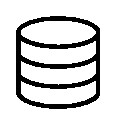
\includegraphics{./figs/icons/database.eps}};
  \node [scale=1,right=2cm of do](sp){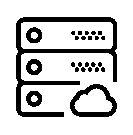
\includegraphics{./figs/icons/server.eps}};
  \node [scale=2,right=2cm of sp](client){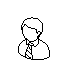
\includegraphics{./figs/icons/user.eps}};
  \draw[-latex] (do.east) -- (sp.west) node [midway,above,font=\scriptsize] {Data \& ADS};
  \draw[-latex,transform canvas={yshift=0.5ex}] (client.west) -- (sp.east) node [midway,above,font=\scriptsize] {Queries};
  \draw[-latex,transform canvas={yshift=-0.5ex}] (sp.east) -- (client.west) node [midway,below,font=\scriptsize] {Results \& VO};
  \node [font=\footnotesize,below=0cm of sp](sp-label){\textbf{Services Provider (SP)}};
  \node [font=\footnotesize] at (do |- sp-label) {\textbf{Data Owner (DO)}};
  \node [font=\footnotesize] at (client |- sp-label) {\textbf{Clients}};
\end{tikzpicture}

        \caption{System Model}
      \end{figure}
    \item \textcolor{Red}{Security Threats}: SP cannot be fully trusted $\Rightarrow$ Query result integrity not guaranteed
    \item \textcolor{Green}{Solution}:
      \begin{itemize}[<1->]
        \item DO signs a well-designed \alert{\emph{authenticated data structure} (ADS)}
        \item SP constructs a cryptographic proof a.k.a.\ \alert{\emph{verifciation object} (VO)}
        \item Clients verify the correctness of the results based on VO
      \end{itemize}
  \end{itemize}
\end{frame}

\begin{frame}{Related Works}
  \begin{columns}
    \begin{column}{0.8\linewidth}
      \begin{itemize}[<+->]
        \item There are two approaches to support authenticated query processing
        \item \alert{ADS-based Solutions}
          \begin{itemize}[<1->]
            \item Designed specifically based on the computation task
            \item \makebox[.35\linewidth][l]{\textcolor{Green}{Pros}: efficient}
              \textcolor{Red}{Cons}: only work for the specific queries
            \item \textcolor{Violet}{Examples}:
              \parbox[t]{\linewidth}{%
                \strut%
                signature chaining~\cite{10.1109/ICDE.2004.1320027}, Merkle hash tree~\cite{10.1007/0-387-34805-0_21}, \\ set accumulator~\cite{10.1145/2660267.2660373}, etc.%
                \strut%
              }%
          \end{itemize}
        \item \alert{General-Purpose Solutions}
          \begin{itemize}[<1->]
            \item Modeling computation task as boolean or arithmetic circuit
            \item \makebox[.35\linewidth][l]{\textcolor{Green}{Pros}: expressive}
              \textcolor{Red}{Cons}: high setup \& proving cost
            \item \textcolor{Violet}{Examples}: zkSNARKs~\cite{10.1109/sp.2013.47}, RAM-based VC~\cite{10.1145/2517349.2522733}, etc.
          \end{itemize}
        \item We focus on \alert{ADS-based solutions} in this dissertation
      \end{itemize}
    \end{column}%
    \begin{column}{0.2\linewidth}
      \begin{figure}
        \onslide<2->{%
          \resizebox{\linewidth}{!}{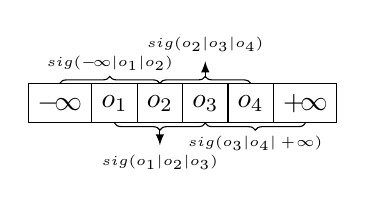
\begin{tikzpicture}
    \tikzstyle{chain-node}=[
        rectangle split,
        rectangle split horizontal,
        rectangle split ignore empty parts,
        rectangle split parts=6,
        draw
    ]
    \node[chain-node] (chain) {
        \nodepart{one} $-\!\infty$
        \nodepart{two} $o_1$
        \nodepart{three} $o_2$
        \nodepart{four} $o_3$
        \nodepart{five} $o_4$
        \nodepart{six} $+\!\infty$
    };

    \draw[decorate, decoration={brace}]
    (chain.one north) -- coordinate (s1) (chain.three north);
    \node[above=1pt of s1,font=\tiny] (s1-label) {$sig(-\!\infty|o_1|o_2)$};

    \draw[decorate, decoration={brace,mirror}]
    (chain.two south) -- coordinate[below=2pt] (s2) (chain.four south);
    \node[below=6pt of s2,font=\tiny] (s2-label) {$sig(o_1|o_2|o_3)$};
    \draw[-latex] (s2) -- (s2-label);

    \draw[decorate, decoration={brace}]
    (chain.three north) -- coordinate[above=2pt] (s3) (chain.five north);
    \node[above=6pt of s3,font=\tiny] (s3-label) {$sig(o_2|o_3|o_4)$};
    \draw[-latex] (s3) -- (s3-label);

    \draw[decorate, decoration={brace,mirror}]
    (chain.four south) -- coordinate (s4) (chain.six south);
    \node[below=1pt of s4,font=\tiny] (s4-label) {$sig(o_3|o_4|+\!\infty)$};
\end{tikzpicture}
}
          \caption{Signature Chaining}
          \resizebox{\linewidth}{!}{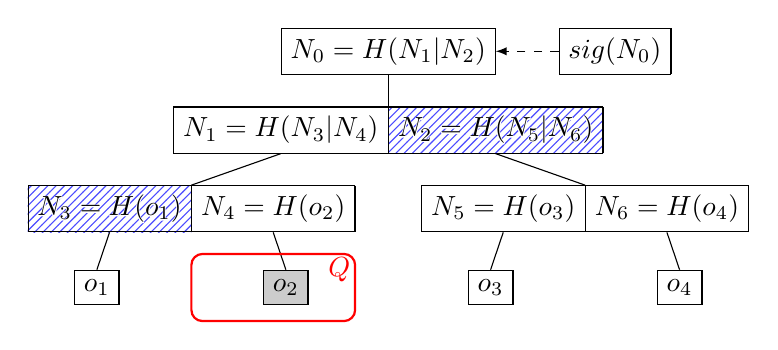
\begin{tikzpicture}
    \tikzstyle{tree node}=[
        rectangle split,
        rectangle split horizontal,
        rectangle split ignore empty parts,
        draw
    ]
    \tikzstyle{tree}=[
        every node/.style={tree node},
        edge from parent path={},
        level/.style={level distance=1cm},
        level 2/.style={sibling distance=5cm},
        level 3/.style={sibling distance=2.4cm},
    ]

    \path[tree] node (root) {$N_0 = H(N_1|N_2)$}
    child {
        node (l1) {
            \nodepart{one} $N_1 = H(N_3|N_4)$ \nodepart{two} \contour{white}{$N_2 = H(N_5|N_6)$}
        }
        child {
            node (l21) {
                \nodepart{one} \contour{white}{$N_3 = H(o_1)$} \nodepart{two} $N_4 = H(o_2)$
            }
            child {node (o1) {$o_1$}}
            child {node [fill=black!20, text=black] (o2) {$o_2$}}
        }
        child {
            node (l22) {
                \nodepart{one} $N_5 = H(o_3)$ \nodepart{two} $N_6 = H(o_4)$
            }
            child {node (o3) {$o_3$}}
            child {node (o4) {$o_4$}}
        }
    };

    \begin{pgfonlayer}{background}
        \fill[pattern=north east lines,pattern color=blue!70]
        (l21.north west) rectangle (l21.one split south);
        \fill[pattern=north east lines,pattern color=blue!70]
        (l1.one split north) rectangle (l1.south east);
    \end{pgfonlayer}

    \foreach \a/\b in {
        root.south/l1,
        l1.one south/l21,
        l1.two south/l22,
        l21.one south/o1,
        l21.two south/o2,
        l22.one south/o3,
        l22.two south/o4%
    }
    \draw [style=edge from parent] (\a) -- (\b.north);

    \node[tree node,right=0.8cm of root] (data) {$sig(N_0)$};
    \draw[dashed,-latex] (data) -- (root);

    \draw [Red,rounded corners,thick]
    let \p1 = ($(o2.south east -| l21.one split) - (0, 0.2)$),
    \p2 = ($(o2.north west -| l21.east) + (0, 0.2)$) in
    (\x1, \y1) rectangle (\x2, \y2)
    node[xshift=-0.2cm, yshift=-0.2cm] {$Q$};
\end{tikzpicture}
}
          \caption{Merkle Hash Tree}
          \onslide<3->{%
            \resizebox{\linewidth}{!}{\begin{tikzpicture}
  \node[matrix] (circuit) {
    \node (circuit-fig) {%
      \begin{tikzpicture}[scale=0.2]
        \node[circle,draw=black,minimum size=10,inner sep=0] (g1) at (0, 0) {};
        \node[circle,draw=black,minimum size=10,inner sep=0] (g2) at (-1, 2) {};
        \node[circle,draw=black,minimum size=10,inner sep=0] (g3) at (1, 2) {};
        \draw (g1) -- (0, -1.5);
        \draw (g1) -- (g2);
        \draw (g1) -- (g3);
        \draw (g2) -- (-0.25, 4);
        \draw (g2) -- (-2, 4);
        \draw (g3) -- (0.25, 4);
        \draw (g3) -- (2, 4);
      \end{tikzpicture}
    };
    \node[below=0cm of circuit-fig] {Circuit};
    \\
  };

  \node[matrix, left=0.2cm of circuit] (input) {
    \node (db) {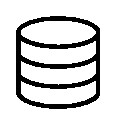
\includegraphics[width=0.6cm]{./figs/icons/database.eps}};
    \node[left=0cm of db] {Data};
    \node[below=0.6cm of db] (sql) {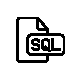
\includegraphics[width=0.6cm]{./figs/icons/sql.eps}};
    \node[left=0cm of sql] {Program};
    \draw[decorate,decoration={brace,amplitude=10pt}]
    (db.east) -- coordinate[right=10pt] (input-mid) (sql.east);
    \\
  };
  \draw[-latex] (input-mid) -- (circuit);

  \node[matrix,right=0.5cm of circuit] (proof) {
    \node (cert) {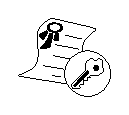
\includegraphics[width=0.7cm]{./figs/icons/cert.eps}};
    \node[below=0cm of cert] {Proof};
    \\
  };
  \draw[-latex] (circuit) -- (proof);
\end{tikzpicture}
}
            \caption{zkSNARKs}
          }
        }
      \end{figure}%
    \end{column}
  \end{columns}
\end{frame}

\begin{frame}{Limitations of the Existing Works}
  \begin{itemize}[<+->]
    \item However, the prior works have only considered \alert{limited query types}
    \item They fail to consider:
      \begin{itemize}[<+- | alert@+>]
        \item Aggregate queries over set-valued data for data analytics
        \item Enforcing fine-grained access control
        \item Query processing in distributed settings
      \end{itemize}
  \end{itemize}

  \begin{columns}[b,onlytextwidth]
    \begin{column}{0.33\linewidth}
      \begin{figure}
        \onslide<3->{%
          \resizebox{\linewidth}{!}{\begin{tikzpicture}
  \node[matrix,ampersand replacement=\&] (input) {
    \node (data) {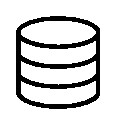
\includegraphics[width=0.5cm]{./figs/icons/database.eps}};
    \node[right=0 of data,scale=0.5] (table) {
      \begin{tabular}{|l|l|}
        \hline
        $o_1$ & $\{a, b, c\}$ \\
        \hline
        $o_2$ & $\{a, d\}$ \\
        \hline
        $\cdots$ & $\cdots$ \\
        \hline
      \end{tabular}
    };
    \\
  };
  \node[right=0.5cm of input] (out) {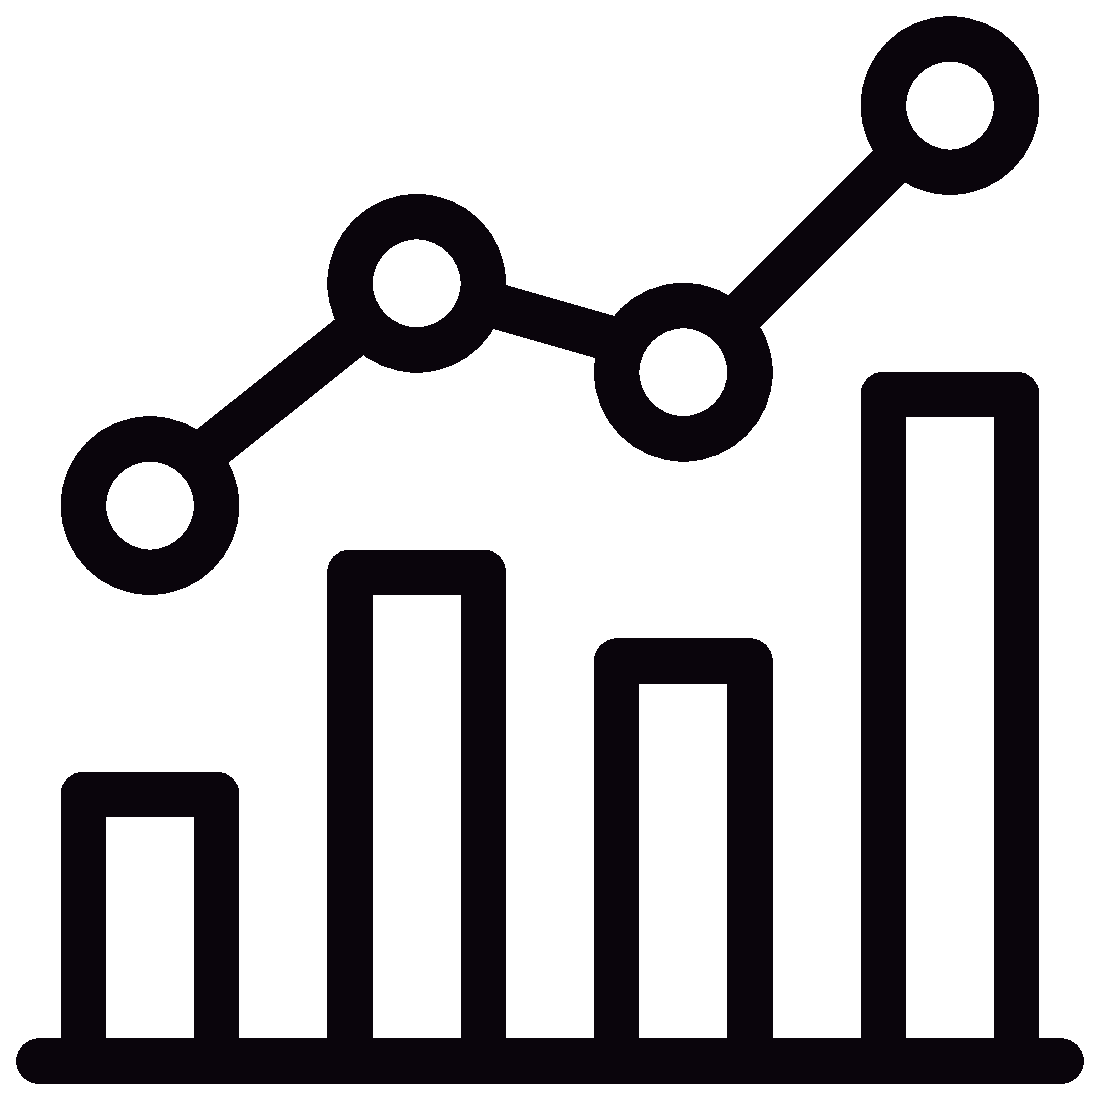
\includegraphics[width=0.5cm]{./figs/icons/analytics.eps}};
  \draw[-latex] (input) -- (out);
\end{tikzpicture}
}
          \caption{Analytical Queries}
        }
      \end{figure}
    \end{column}
    \begin{column}{0.33\linewidth}
      \begin{figure}
        \onslide<4->{%
          \resizebox{\linewidth}{!}{\begin{tikzpicture}
  \node[matrix, inner sep=0] (output) {
    \node[scale=0.9] at (0,0.5) (user1) {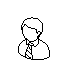
\includegraphics{figs/icons/user.eps}};
    \node[scale=0.9] at (0,-0.5) (user2) {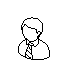
\includegraphics{figs/icons/user.eps}};
    \node[right=0cm of user1] (user1-info) {$u_1: \{Role_A, Role_B\}$};
    \node[right=0cm of user2] (user2-info) {$u_2: \{Role_C\}$};
    \\
  };

  \coordinate (user-mid) at ($(user1)!.5!(user2)$);
  \node[left=2cm of user-mid] (input) {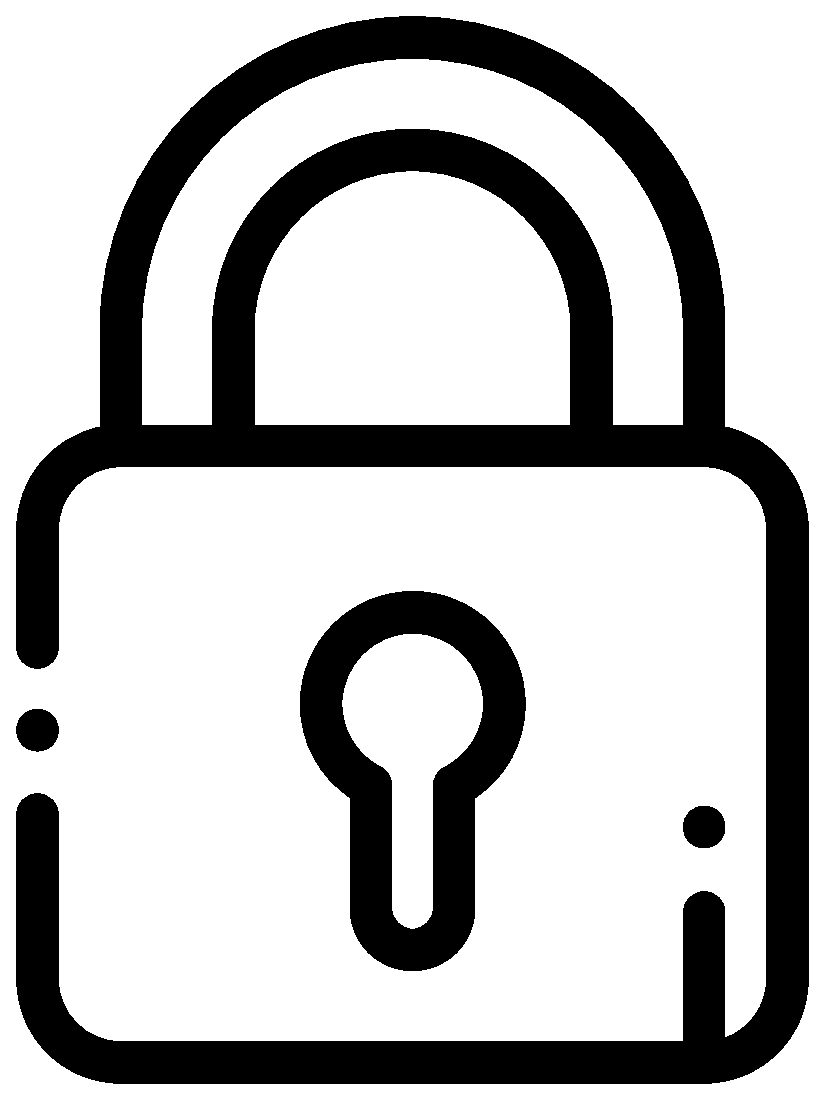
\includegraphics[width=0.5cm]{figs/icons/lock.eps}};
  \node[below=0cm of input] {$\Upsilon = Role_A $};
  \coordinate (mid) at ($(input)!.4!(user-mid)$);
  \draw (input.east) -- (mid);
  \draw[-latex] (mid) |- (user1.west) node[pos=0.75, sloped, scale=1, color=Green] {\ding{52}};
  \draw[-latex] (mid) |- (user2.west) node[pos=0.75, sloped, scale=1, color=Red] {\ding{55}};
\end{tikzpicture}
}
          \caption{Access Control}
        }
      \end{figure}
    \end{column}
    \begin{column}{0.33\linewidth}
      \begin{figure}
        \onslide<5->{%
          \resizebox{\linewidth}{!}{\begin{tikzpicture}
  \node[matrix,inner sep=0.01cm,draw=black,ellipse,dashed] (server) {%
    \node (s1) {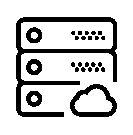
\includegraphics[width=0.5cm]{./figs/icons/server.eps}};
    \node[below=0 of s1.south east, anchor=north west] (s2) {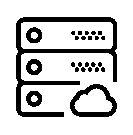
\includegraphics[width=0.5cm]{./figs/icons/server.eps}};
    \node[below=0 of s1.south west, anchor=north east] (s3) {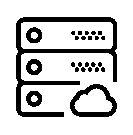
\includegraphics[width=0.5cm]{./figs/icons/server.eps}};
    \\
  };

  \node[scale=0.9,left=2cm of server] (user) {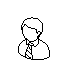
\includegraphics{./figs/icons/user.eps}};
  \draw[-latex] (user) -- (server) node[midway, above, color=Red] {$q: \langle k, loc \rangle$};
\end{tikzpicture}
}
          \caption{Distributed Query Processing}
        }
      \end{figure}
    \end{column}
  \end{columns}
\end{frame}

\section{Authenticating Aggregate Queries over Set-Valued Data}

\subsection{Problem Formulation}

\begin{frame}[fragile]{Example of Aggregate Queries over Set-Valued Data}
  \begin{columns}[onlytextwidth]
    \begin{column}{.5\linewidth}
      \setbeamercovered{transparent}
      \begin{table}
        \resizebox{\linewidth}{!}{%
          \begin{tabular}{ccl}
            \toprule
            \textbf{PID} & \textbf{ZIP} & \multicolumn{1}{c}{\textbf{Mut-Genes}}\\
            \midrule
            \onslide<1,2,3>{P1&95014&\alert<2>{A-C130R}, P-I696M} \\
            \onslide<1,3,4>{P2&20482&H-C282Y, \alert<4>{P-P12A}, \alert<3,4>{R-G1886S}} \\
            \onslide<1,2,3>{P3&95014&\alert<2>{A-C130R}, U-G71R, W-R611H} \\
            \onslide<1,3>{P4&01720&A-V2050L, H-C282Y, M-R52C, U-G71R} \\
            \onslide<1,3,4>{P5&20134&A-C130R, \alert<4>{P-P12A}, \alert<3,4>{R-G1886S}, S-E366K} \\
            \onslide<1,3>{P6&17868& C-R102G, \alert<3>{R-G1886S}} \\
            \onslide<1,3>{P7&55410&C-R102G, C-Q1334H, S-E288V} \\
            \onslide<1,3,4>{P8&20852&C-R102G, \alert<4>{P-P12A}, \alert<3,4>{R-G1886S}, K-T220M} \\
            \bottomrule
          \end{tabular}
        }
        \caption{Set-Valued Genome Dataset~\cite{pgp}}
      \end{table}
    \end{column}%
    \begin{column}{.5\linewidth}
      \begin{itemize}[<+(1)->]% chktex 36
        \item \textbf{Q1}: Find the most common gene in the district of Cupertino, CA (ZIP\@: 95014) \\
          \textcolor{Violet}{\emph{Answer:} \{`A-C130R'\}}
        \item \textbf{Q2}: Count the number of participants who carry the gene `R-G1886S' \\
          \textcolor{Violet}{\emph{Answer:} 4}
        \item \textbf{Q3}: Find the most frequent genes with supports $\ge$ 3 in ZIPs 20*** \\
          \textcolor{Violet}{\emph{Answer:} \{`P-P12A', `R-G1886S'\}}
      \end{itemize}
    \end{column}
  \end{columns}
\end{frame}

\begin{frame}{Problem Definition}
  \begin{itemize}[<+->]
    \item \textbf{Dataset} $\mathbb{D} = \{o_1, o_2, \dotsc, o_n\}$
      \begin{itemize}[<.->]
        \item $o_i = \langle A_i, X_i \rangle$.
        \item $A_i$ is a set of \textcolor{Green}{non-sensitive} attributes
        \item $X_i$ is a \textcolor{Red}{sensitive} multiset of \emph{features}
      \end{itemize}
    \item \textbf{Aggregate Query} $Q = (q, \{x_i\}, [\alpha, \beta])$
      \begin{itemize}[<.->]
        \item $q$ is an aggregate operator, i.e., \emph{max/min}, \emph{count}, \emph{sum}, \emph{top-$k$}, and \emph{frequent feature query (FFQ)}
        \item $\{x_i\}$ is the queried feature specified for \emph{count} and \emph{sum}
        \item $[\alpha, \beta]$ specifies the selection range over the \textcolor{Green}{non-sensitive} attributes
      \end{itemize}
    \item \textbf{Threat Model}
      \begin{itemize}[<.->]
        \item \alert{Integrity}: SP should prove the \emph{soundness} and \emph{completeness} of the results
        \item \alert{Confidentiality}: Clients should not infer any \emph{sensitive source data}
      \end{itemize}
  \end{itemize}
\end{frame}

\subsection{Preliminaries}

\begin{frame}{Preliminaries}
  \begin{definition}<+->[Bilinear-Map (BM) Accumulator]
    Let $g$ be the group generator of a cyclic multiplicative group $\mathbb{G}$ and $s$ be a \textcolor{Red}{private value of DO}. The accumulator maps a multiset $X = \{ x_1, x_2, \dotsc, x_m \}$ to a single value in $\mathbb{G}$:
    \begin{align*}
      acc(X) = g^{P(X)} = g^{\prod_{x_i \in X}(x_i + s)}
    \end{align*}
    Without knowing $s$, one can still compute an $acc(\cdot)$ value by giving $g^s, g^{s^2}, \dotsc$
  \end{definition}
  \begin{example}<.->
    $X = \{ 1, 1, 2 \}$, $acc(X) = g^{{(1+s)}^2(2+s)} = g^{s^3+4 s^2+5 s+2} = g^{s^3} \cdot {(g^{s^2})}^4 \cdot {(g^s)}^5 \cdot g^2$
  \end{example}
  \begin{definition}<+->[Randomized BM Accumulator]
    BM accumulator is \alert{deterministic} for \emph{a fixed multiset}. As such, an adversary can tell in high confidence that two multisets are the same. We can randomize BM accumulator as following:
    \begin{align*}
      acc(X) = g^{P(X) \cdot r_X} = g^{r_X\prod_{x_i \in X}(x_i + s)}
    \end{align*}
    $r_X$ is a random value \textcolor{Red}{hidden from Clients} but \textcolor{Green}{disclosed to SP}.
  \end{definition}
\end{frame}

\begin{frame}{Preliminaries}
  \begin{definition}[Cryptographic Hash Function]
    A cryptographic hash function $H(\cdot)$ accepts an arbitrary-length string as its input and returns a fixed-length bit string such that it is computationally infeasible to find $m_1 \neq m_2$ and $H(m_1) = H(m_2)$.
  \end{definition}
  \begin{definition}[Bilinear Pairing]
    Let $\mathbb{G}, \mathbb{G}_T$ be two cyclic multiplicative groups of order $p$.
    A pairing is a map $e: \mathbb{G} \times \mathbb{G} \to \mathbb{G}_T$, which satisfies:
    \begin{itemize}
      \item \textbf{Bilinearity}: $e(u^a,v^b) = {e(u,v)}^{ab}$, $\forall u, v \in \mathbb{G}$
      \item \textbf{Non-degeneracy}: $e(g,g) \ne 1$
      \item \textbf{Computability}: Given $u, v \in \mathbb{G}$, it is easy to compute $e(u, v)$
    \end{itemize}
  \end{definition}
\end{frame}

\subsection{PA$^2$ Authentication Framework}

\begin{frame}[fragile]{PA$^2$ Authentication Framework Overview}
  \begin{figure}
    \onslide<+->{%
      \resizebox{.8\linewidth}{!}{%
        \begin{tikzpicture}
          \node[anchor=south west,inner sep=0] (A) at (0,0)
            {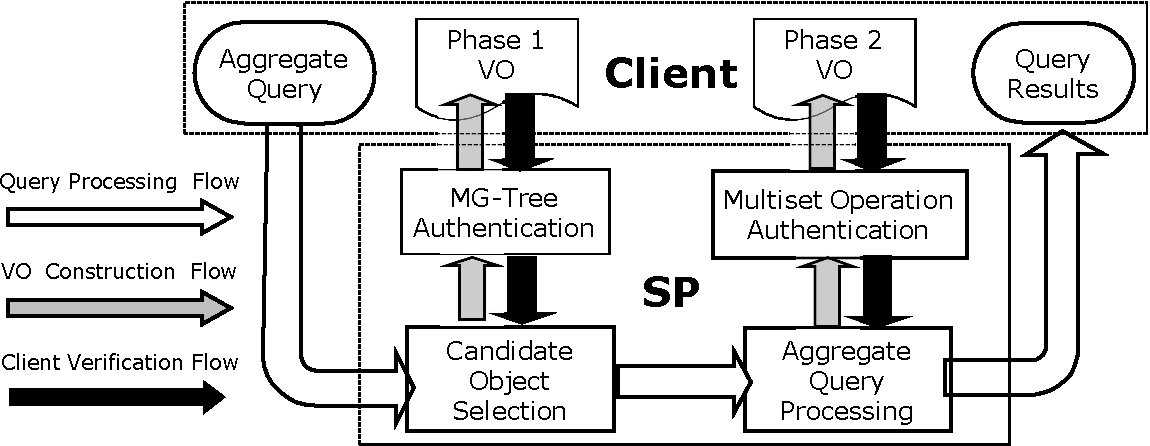
\includegraphics[width=\linewidth]{figs/aggregate-queries/overview.pdf}};
          \coordinate (multiset1) at (8.6,2.2);
          \coordinate (multiset2) at (11.9,3.45);
          \coordinate (aggregate1) at (9,0.1);
          \coordinate (aggregate2) at (11.7,1.55);
          \coordinate (select1) at (4.8,0.1);
          \coordinate (select2) at (7.57,3.45);
          \draw<2>[Red,ultra thick] (multiset1) rectangle (multiset2);
          \fill<2>[draw=none,fill=black,fill opacity=0.3,even odd rule]
            (A.south west) rectangle (A.north east)
            (multiset1) rectangle (multiset2);
          \draw<3>[Red,ultra thick] (aggregate1) rectangle (aggregate2);
          \fill<3>[draw=none,fill=black,fill opacity=0.3,even odd rule]
            (A.south west) rectangle (A.north east)
            (aggregate1) rectangle (aggregate2);
          \draw<4>[Red,ultra thick] (select1) rectangle (select2);
          \fill<4>[draw=none,fill=black,fill opacity=0.3,even odd rule]
            (A.south west) rectangle (A.north east)
            (select1) rectangle (select2);
        \end{tikzpicture}
      }
      \caption{Privacy-Preserving Authentication Framework for Aggregate Queries}
    }
  \end{figure}
  \begin{itemize}[<+- | alert@+>]
    \item PA$^2$ Protocols on Multiset Operations
    \item PA$^2$ Algorithms on Aggregate Queries
    \item PA$^2$ on Candidate Object Selection
  \end{itemize}
\end{frame}

\subsubsection{PA$^2$ Protocols on Multiset Operations}

\begin{frame}{PA$^2$ Protocols on Multiset Operations --- Subset}
  \begin{block}{$sub(X_1, X_2)$: returns $acc$ value of $X_1 - X_2$ iff $X_2 \subseteq X_1$}
    \begin{itemize}
      \item DO prepares $acc(X_1)$, $acc(X_2)$
      \item SP computes ${acc(X_1 - X_2)}^* = g^{r_{X_1}/r_{X_2} \prod_{x \in (X_1 - X_2)} (x+s)}$
      \item Client verifies $e(acc(X_2), {acc(X_1 - X_2)}^*) \stackrel{?}{=} e(acc(X_1), g)$
    \end{itemize}
  \end{block}
  \begin{example}
    \begin{itemize}
      \item $X_1 = \{ 1, 1, 2 \}$, $X_2 = \{ 1, 2 \}$
      \item $acc(X_1) = g^{r_{X_1}{(1+s)}^2(2+s)}$, $acc(X_2) = g^{r_{X_2}(1+s)(2+s)}$, ${acc(X_1 - X_2)}^* = g^{r_{X_1}/r_{X_2}(1+s)}$
      \item \(
        \begin{aligned}[t]
          e(acc(X_2), {acc(X_1 - X_2)}^*) &= e(g^{r_{X_2}(1+s)(2+s)},g^{r_{X_1}/r_{X_2}(1+s)}) = {e(g, g)}^{r_{X_1}{(1+s)}^2(2+s)} \\
          e(acc(X_1), g) &=  e(g^{r_{X_1}{(1+s)}^2(2+s)}, g) = {e(g, g)}^{r_{X_1}{(1+s)}^2(2+s)}
        \end{aligned}
        \)
    \end{itemize}
  \end{example}
\end{frame}

\begin{frame}{PA$^2$ Protocols on Multiset Operations --- Sum}
  \begin{block}{$sum(\{X_1, \dotsc, X_n\})$: returns $acc$ value of $S = \uplus_{i=1}^n X_i$}
    \begin{itemize}
      \item DO prepares $acc(X_1), \dotsc, acc(X_n)$
      \item SP computes ${acc(\uplus_{j = 1}^i X_j)}^*$, for $i \in [2, n]$
      \item Client verifies
        \begin{adjustbox}{valign=t}
          \(
          \begin{aligned}
            \left \{
              \begin{array}{l}
                e(acc(X_1), acc(X_2)) \stackrel{?}{=} e({acc(X_1 \uplus X_2)}^*, g)\\
                e({acc(X_1\uplus X_2)}^*, acc(X_3)) \stackrel{?}{=} e({acc(X_1\uplus X_2\uplus X_3)}^*, g) \\
                \vdots\\
                e({acc(\uplus_{i=1}^{n-1} X_i)}^*, acc(X_n)) \stackrel{?}{=} e({acc(S)}^*, g)
              \end{array}
            \right.
          \end{aligned}
          \)
        \end{adjustbox}
    \end{itemize}
  \end{block}
  \begin{example}
    \begin{itemize}
      \item $X_1 = \{ 1 \}$, $X_2 = \{ 1 \}$, $X_3 = \{ 2 \}$
      \item SP returns ${acc(X_1 \uplus X_2)}^* = acc(\{1, 1\})$ and ${acc(S)}^* = {acc(X_1 \uplus X_2 \uplus X_3)}^* = acc(\{1, 1, 2\})$
    \end{itemize}
  \end{example}
\end{frame}

\begin{frame}{PA$^2$ Protocols on Multiset Operations --- Empty}
  \begin{block}{$empty(\{X_1, \dotsc, X_n\})$: returns whether $\cap_{i=1}^n X_i = \emptyset$}
    \begin{itemize}
      \item DO prepares $acc(X_1), \dotsc, acc(X_n)$
      \item Based on \alert{extended Euclidean algorithm}
        \begin{align*}
          \textstyle%
          \cap \{ X_i \} = \emptyset \Rightarrow \exists Q_i \text{ s.t. } \sum_{i=1}^n Q_i \cdot P(X_i) = 1
        \end{align*}
      \item SP computes $F_i^* = g^{Q_i}$, for $i \in [1, n]$
      \item Client verifies $\prod_{i=1}^n e(acc(X_i), F_i^*) \stackrel{?}{=} e(g, g)$
    \end{itemize}
  \end{block}
  \begin{example}
    \begin{itemize}
      \item $X_1 = \{ 1 \}$, $X_2 = \{ 2 \}$
      \item SP returns $F_1^* = g^{-1/r_{X_1}}$, $F_2^* = g^{1/r_{X_2}}$
      \item \(
        \begin{aligned}[t]
          e(acc(X_1), F_1^*)e(acc(X_2), F_2^*) &= e(g^{r_{X_1}(1+s)}, g^{-1/r_{X_1}})e(g^{r_{X_2}(2+s)}, g^{1/r_{X_2}}) \\
                                               &= {e(g,g)}^{-1-s}{e(g,g)}^{2+s} = {e(g,g)}^{-1-s+2+s} = e(g,g)
        \end{aligned}
        \)
    \end{itemize}
  \end{example}
\end{frame}

\begin{frame}{PA$^2$ Protocols on Multiset Operations --- Union}
  \begin{block}{$union(\{X_1, \dotsc, X_2\})$: returns $acc$ value of $U = \cup_{i=1}^n X_i$}
    \begin{itemize}
      \item Denote $\widehat{X}_i$ as the \alert{set version} of a multiset $X_i$.
      \item Client verifies two conditions:
        \begin{enumerate}
          \item \alert{Deflation checking} (no object is missing):
            \begin{align*}
              \widehat{X}_1 \subseteq U \wedge \widehat{X}_2 \subseteq U \wedge \cdots \widehat{X}_n \subseteq U
            \end{align*}
          \item \alert{Inflation checking} (no non-result object is added):
            \begin{align*}
              (U - \widehat{X}_1) \cap (U - \widehat{X}_2) \cap \cdots (U - \widehat{X}_n) = \emptyset
            \end{align*}
        \end{enumerate}
    \end{itemize}
  \end{block}
  \begin{example}
    \begin{itemize}
      \item $X_1 = \{ 1 \}$, $X_2 = \{ 2 \}$, $U = \{ 1, 2 \}$
      \item \alert{Deflation checking}: $\{1\} \subseteq \{1,2\}, \{2\} \subseteq \{1,2\}$ \\
        \alert{Inflation checking}: $\{2\} \cap \{1\} = \emptyset$
    \end{itemize}
  \end{example}
\end{frame}

\begin{frame}{PA$^2$ Protocols on Multiset Operations --- Times}
  \begin{block}{$times(X, t)$: returns $acc$ value of $t \cdot X$}
    \begin{itemize}
      \item Let $d = \lfloor \log_2(t) \rfloor$ and $t = {(b_0b_1\cdots b_d)}_2$, the \alert{binary form} of $t$.
      \item $times(X, t) = sum(\{b_0 \cdot X, \dotsc, b_i \cdot 2^i \cdot X, \dotsc, b_d \cdot 2^d \cdot X\})$
      \item SP computes ${acc(2\cdot X)}^*, \dotsc, {acc({2^d} \cdot X)}^*, {acc(t \cdot X)}^*$
      \item Client verifies:
        \begin{itemize}
          \item $e({acc(2^{i-1} \cdot X)}^*, {acc(2^{i-1} \cdot X)}^*) = e({acc(2^{i} \cdot X)}^*, g)$, for $i \in [1, d]$
          \item Apply $sum(\{b_0 \cdot X, \dotsc, b_i \cdot 2^i \cdot X, \dotsc, b_d \cdot 2^d \cdot X\})$
        \end{itemize}
    \end{itemize}
  \end{block}
  \begin{example}
    \begin{itemize}
      \item When $t = 5$, SP computes $acc(2\cdot X), acc(4\cdot X)$
      \item $acc(5 \cdot X) = sum(\{X, 4\cdot X\})$
    \end{itemize}
  \end{example}
\end{frame}

\subsubsection{PA$^2$ Algorithms on Aggregate Queries}

\begin{frame}{PA$^2$ Algorithms on Aggregate Queries --- Sum Query}
  \begin{block}{Sum Query $sum(x_q)$: returns feature $x_q$'s multiplicity sum $\eta_q$}
    \begin{itemize}
      \item Denote $X_1, \dotsc, X_n$ as input multisets and $R = \{ (x_q, \eta_q) \}$ as the result.
      \item Execute $sum(\{X_1, \dotsc, X_n\})$ to get verified $acc(S)$, where $S = \uplus \{X_i\}$
      \item Client verifies two conditions:
        \begin{enumerate}
          \item \alert{Inflation checking} (no non-result object is added):
            \begin{align*}
              R \subseteq S
            \end{align*}
          \item \alert{Deflation checking} (no object is missing):
            \begin{align*}
              (S - R) \cap R = \emptyset
            \end{align*}
        \end{enumerate}
    \end{itemize}
  \end{block}
  \begin{example}
    \begin{itemize}
      \item $S = \{(a,6), (b, 1), (c, 5), (d, 3), (e, 2)\}$, $x_q = a$. The result is $R = \{(a, 6)\}$.
      \item \alert{Inflation checking}: $\{(a, 6)\} \subseteq \{(a,6)$, $(b, 1)$, $(c, 5)$, $(d, 3)$, $(e, 2)\}$ \\
        \alert{Deflation checking}: $\{(b, 1), (c,5), (d, 3), (e, 2)\} \cap \{(a, 6)\} = \emptyset$
    \end{itemize}
  \end{example}
\end{frame}

\begin{frame}{PA$^2$ Algorithms on Aggregate Queries --- Max Query}
  \begin{block}{Max Query: returns the feature with the highest (i.e., top-1) multiplicity}
    \begin{itemize}
      \item Denote $X_1, \dotsc, X_n$ as input multisets and $R = \{ (x, \tau) \}$ as the result.
      \item Execute $sum(\{X_1, \dotsc, X_n\})$ to get verified $acc(S)$, where $S = \uplus \{X_i\}$
      \item Execute $union(\{X_1, \dotsc, X_n\})$ to get verified $acc(U)$, where $U = \cup \{\widehat{X}_i\}$
      \item Client verifies three conditions:
        \begin{enumerate}
          \item \alert{Inflation checking}: $R \subseteq S$
          \item \alert{Deflation checking}: $(S - R) \cap R = \emptyset$
          \item \alert{Completeness checking} (all other features have multiplicity less than $\tau$):
            \begin{align*}
              (S - R) \subseteq \tau \cdot (U -\widehat{R})
            \end{align*}
        \end{enumerate}
    \end{itemize}
  \end{block}
  \begin{example}
    \begin{itemize}
      \item $S = \{(a,6), (b, 1), (c, 5), (d, 3), (e, 2)\}$, $U = \{(a, 1), (b, 1), (c, 1), (d, 1), (e, 1)\}$.
      \item The result is $R = \{(a, 6)\}$.
      \item \alert{Completeness checking}: $\{(b, 1), (c, 5), (d, 3), (e, 2)\} \subseteq $ $\{(b,$ $6), (c, 6), (d, 6), (e, 6)\}$
    \end{itemize}
  \end{example}
\end{frame}

\begin{frame}{PA$^2$ Algorithms on Aggregate Queries --- Other Queries}
  \begin{itemize}
    \item \textbf{Count Query}
      \begin{itemize}
        \item Returns the count of candidate objects that have the queried feature.
        \item Equivalent to \alert{Sum Query} with multiplicity of each feature enforced as 1.
      \end{itemize}
    \item \textbf{Average Query}
      \begin{itemize}
        \item Returns the average multiplicity of queried feature in the candidate objects.
        \item Equivalent to \alert{Sum Query} divided by \alert{Count Query}.
      \end{itemize}
    \item \textbf{Min Query}
      \begin{itemize}
        \item Returns the feature with the lowest (i.e. bottom-$1$) multiplicity.
        \item Similar to \alert{Max Query}, except $(S - R) \supseteq {\tau} \cdot (U - \widehat{R})$.
      \end{itemize}
    \item \textbf{Frequent Features Query}
      \begin{itemize}
        \item Returns the feature with multiplicity larger than threshold $\tau$.
        \item Sub module of \alert{Max Query}.
      \end{itemize}
    \item \textbf{Top-$k$ Query}
      \begin{itemize}
        \item Returns the features with the top-$k$ multiplicity.
        \item Similar to \alert{Max Query}, except $\tau$ is the $k$-th feature's multiplicity.
      \end{itemize}
  \end{itemize}
\end{frame}

\subsubsection{PA$^2$ on Candidate Object Selection}

\begin{frame}{PA$^2$ on Candidate Object Selection}
  \begin{figure}
    \begin{subfigure}[b]{.4\linewidth}
      \centering
      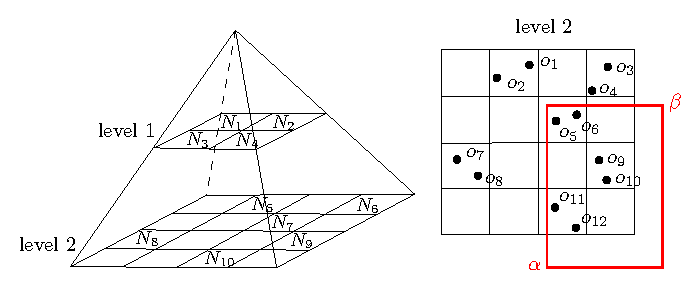
\includegraphics[width=\linewidth]{figs/aggregate-queries/pyramid.eps}
      \caption{Structure}
    \end{subfigure}\quad%
    \begin{subfigure}[b]{.4\linewidth}
      \centering
      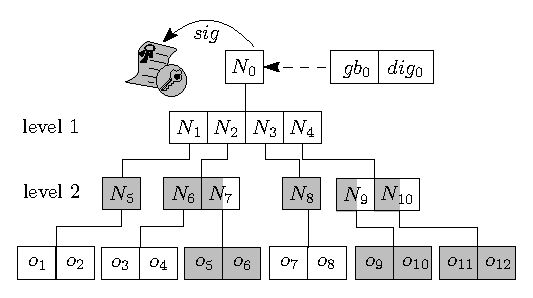
\includegraphics[width=\linewidth]{figs/aggregate-queries/grid_tree.eps}
      \caption{Index}
    \end{subfigure}
    \caption{Merkle Grid Tree (MG-tree)}
  \end{figure}
  \begin{itemize}
    \item \alert{Leaf Node}: $dig_i = H(H(acc(X_{c_1})) | \dotsb | H(acc(X_{c_C})) )$
    \item \alert{Non-Leaf Node}: $dig_i = H(gb_{c_1} | dig_{c_1} | \dotsb | gb_{c_C} | dig_{c_C} )$
    \item Apply \alert{Bucket Indistinguishability} to \emph{preserve privacy}
  \end{itemize}
\end{frame}

\subsection{Performance Evaluation}

\begin{frame}{Performance Evaluation}
  \begin{table}
    \footnotesize
    \begin{tabular}{cccc}
      \toprule
      Dataset & \tabincell{c}{Dataset\\ Size (MB)} & {Setup Time (s)} & \tabincell{c}{MG-tree Index\\Size (MB)} \\
      \midrule
      PGP  & 0.08 & 9.7 & 0.42 \\
      FoodMarket & 0.9 & 136 & 7.1 \\
      TPC-H & 13 & 1,365 & 116 \\
      \bottomrule
    \end{tabular}
    \caption{DO Setup Overhead}
  \end{table}

  \begin{itemize}
    \item Datasets:
      \begin{description}
        \item[PGP] $600$ participants, totally $395$ unique mutation genes (avg. $35$ per person)
        \item[FoodMarket] $\fnum{164558}$ shopping transaction records from $\fnum{8842}$ users and $\fnum{1560}$ products
        \item[TPC-H] $\fnum{1020116}$ transaction records from $\fnum{255000}$ orders and $\fnum{1700}$ suppliers
      \end{description}
  \end{itemize}
\end{frame}

\begin{frame}{Performance Evaluation}
  \savebox{\figbox}{%
    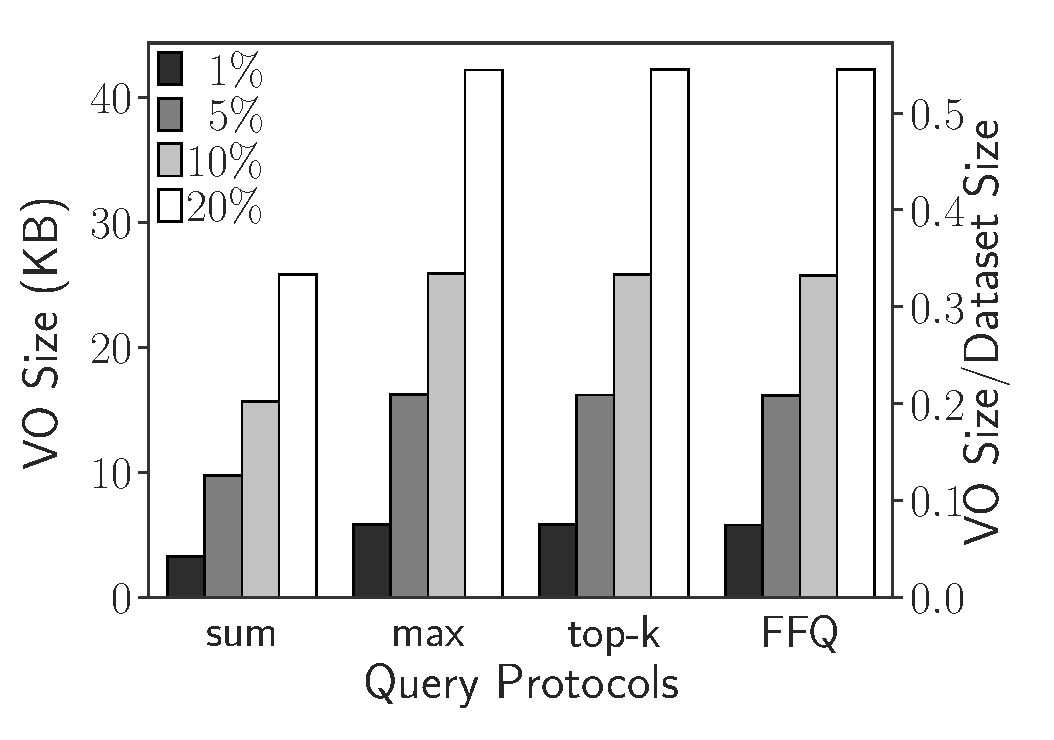
\includegraphics[height=.3\textheight]{exp-figs/aggregate-queries/pgp_vo.eps}%
  }
  \begin{figure}
    \setlength{\tabcolsep}{0pt}
    \renewcommand{\arraystretch}{0}
    \begin{tabular}{c@{\quad}lll}
      PGP &
      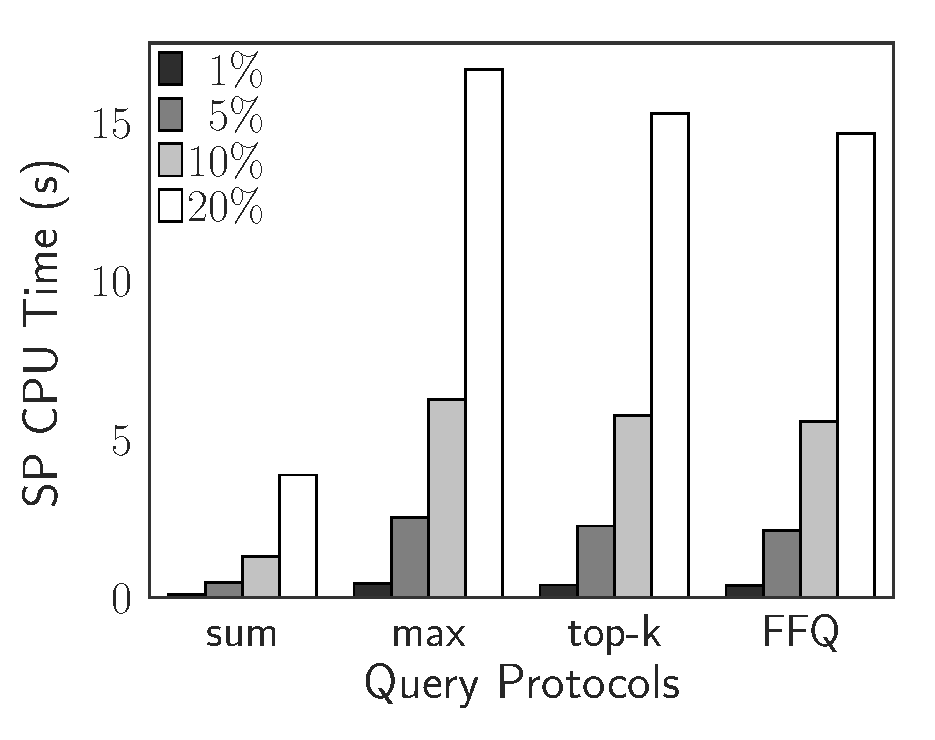
\includegraphics[valign=m,totalheight=\ht\figbox]{exp-figs/aggregate-queries/pgp_sp.eps} &
      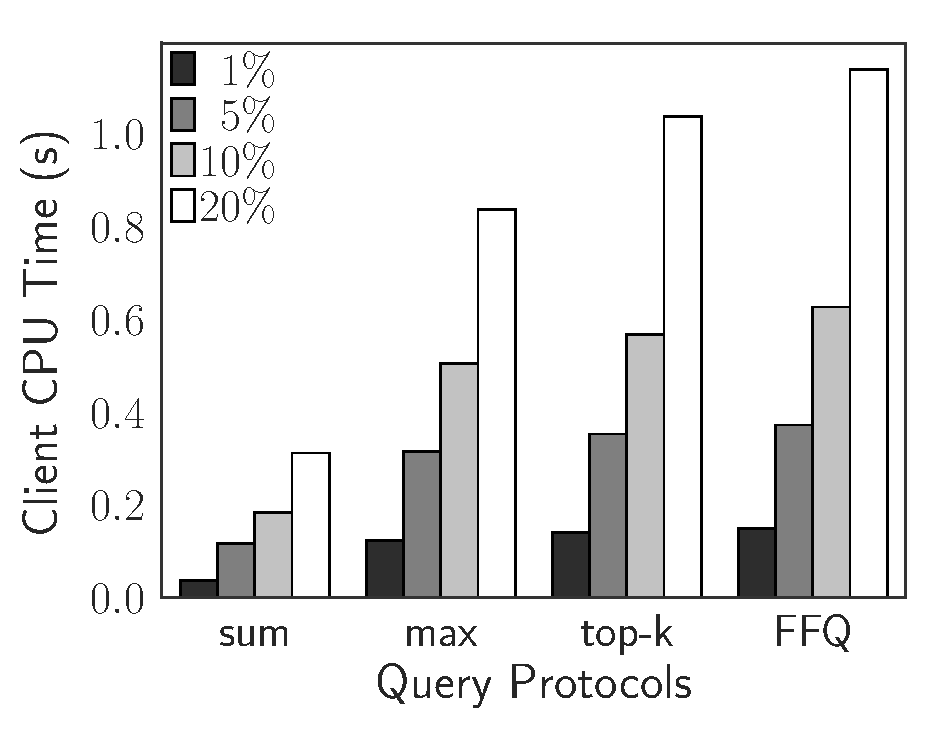
\includegraphics[valign=m,totalheight=\ht\figbox]{exp-figs/aggregate-queries/pgp_client.eps} &
      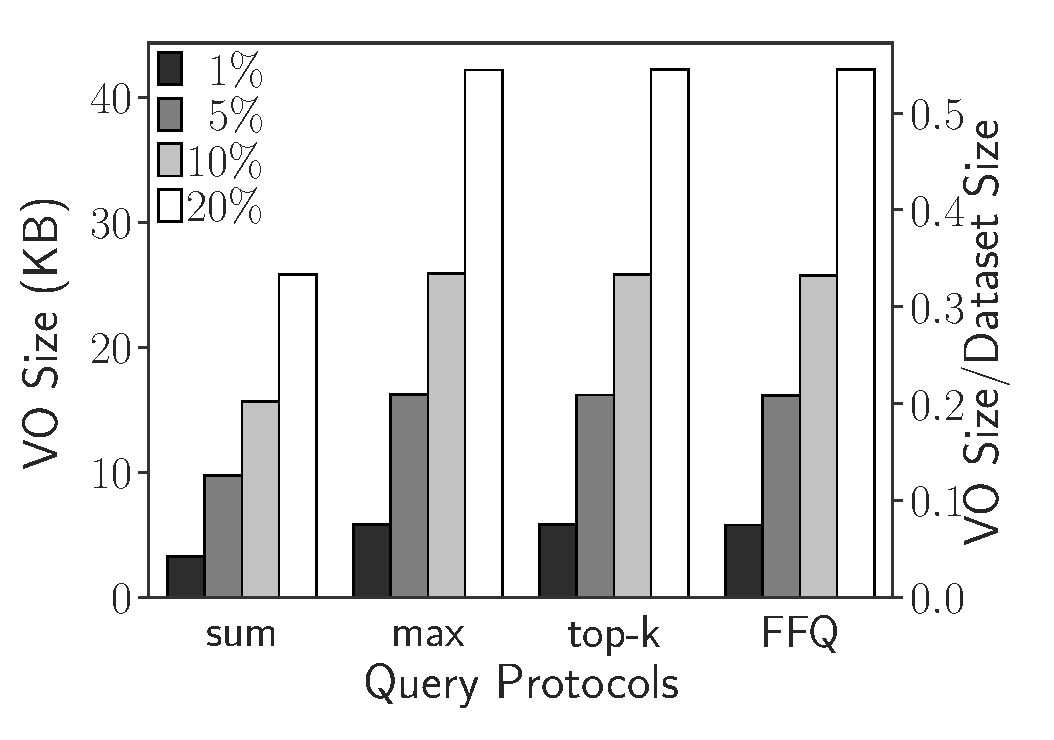
\includegraphics[valign=m,totalheight=\ht\figbox]{exp-figs/aggregate-queries/pgp_vo.eps}
      \\
      FoodMarket &
      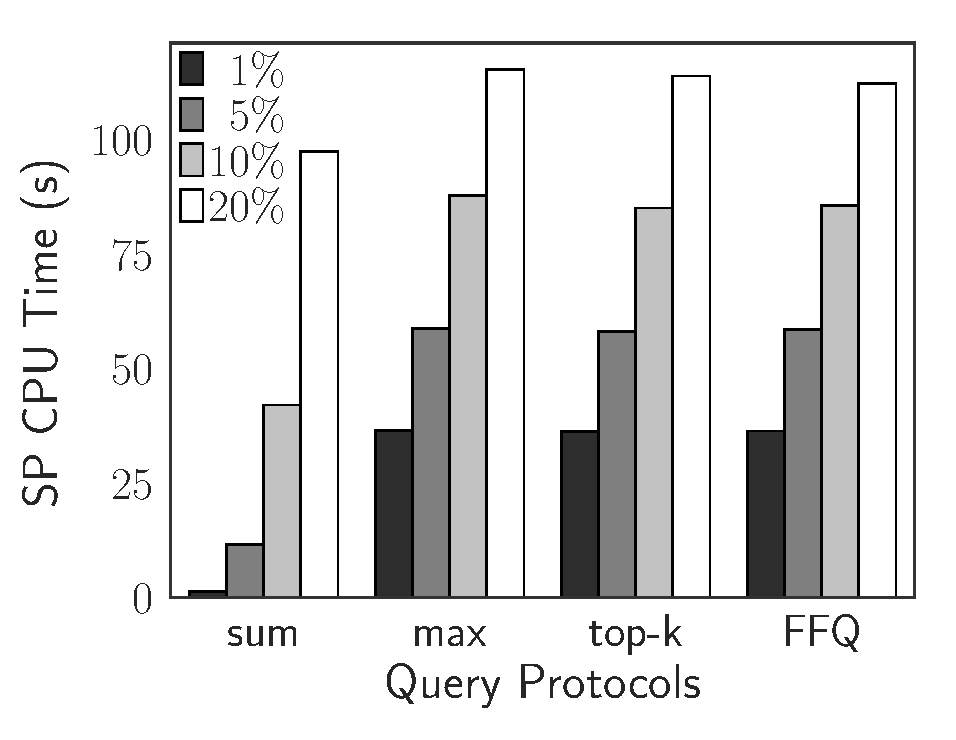
\includegraphics[valign=m,totalheight=\ht\figbox]{exp-figs/aggregate-queries/foodmarket_sp.eps} &
      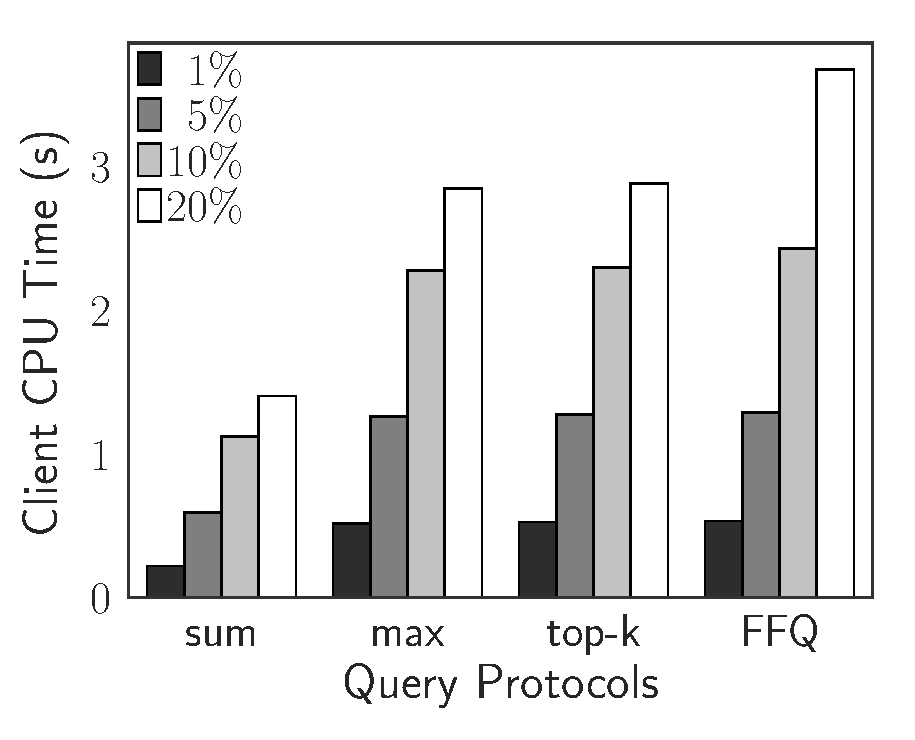
\includegraphics[valign=m,totalheight=\ht\figbox]{exp-figs/aggregate-queries/foodmarket_client.eps} &
      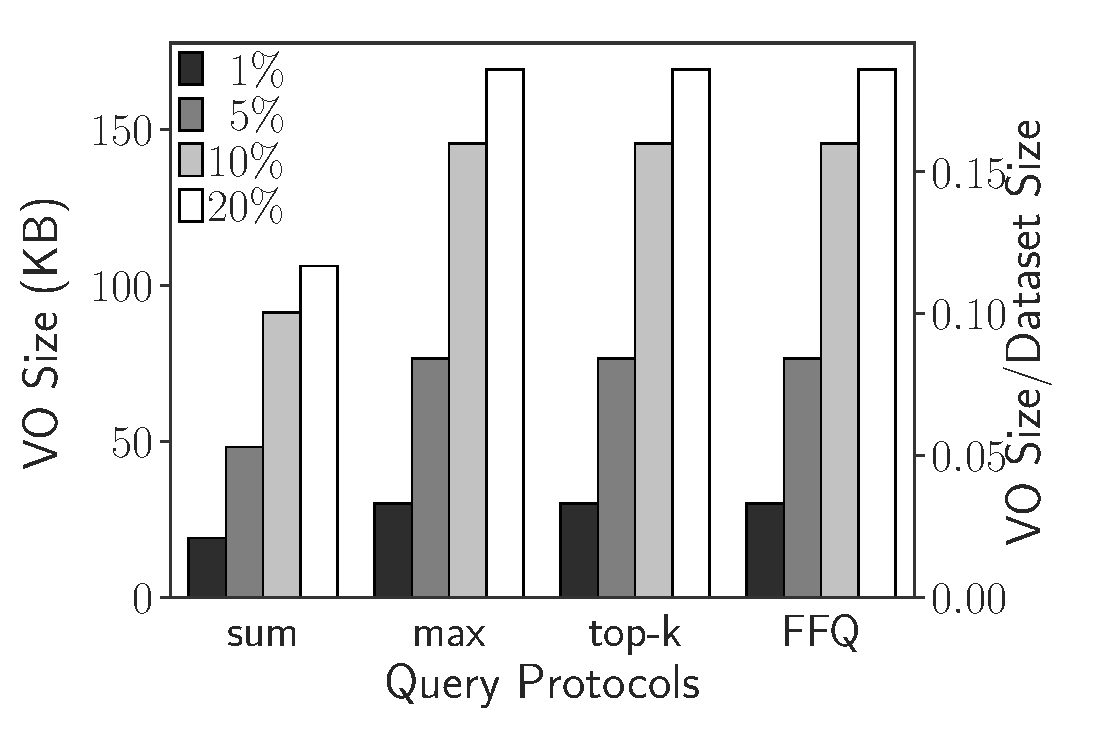
\includegraphics[valign=m,totalheight=\ht\figbox]{exp-figs/aggregate-queries/foodmarket_vo.eps}
      \\
      TPC-H &
      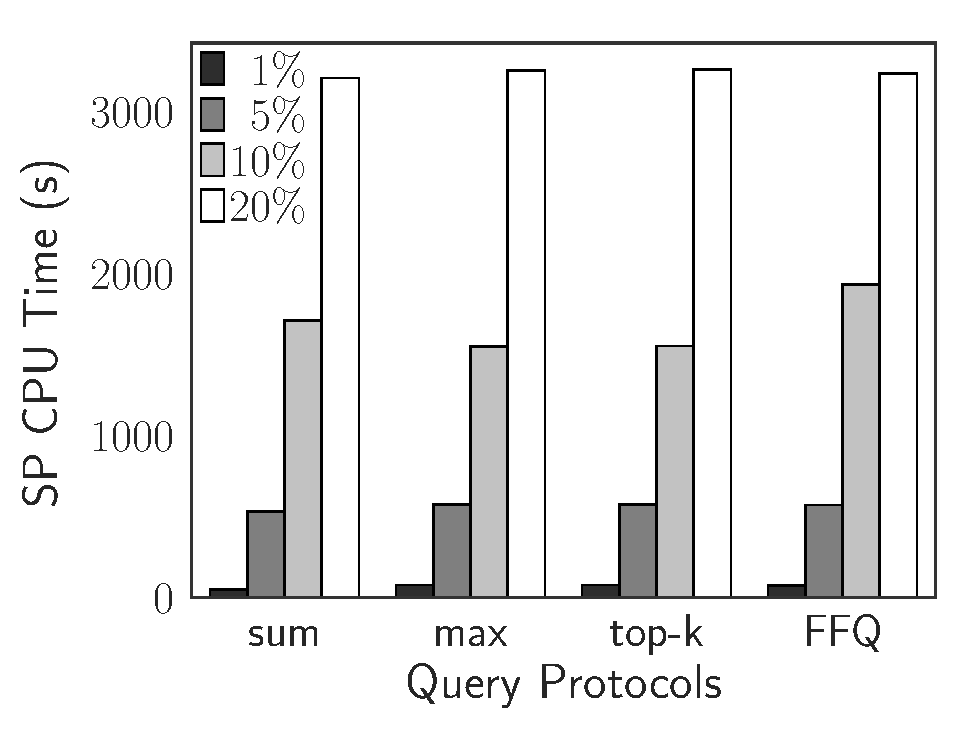
\includegraphics[valign=m,totalheight=\ht\figbox]{exp-figs/aggregate-queries/tpch_sp.eps} &
      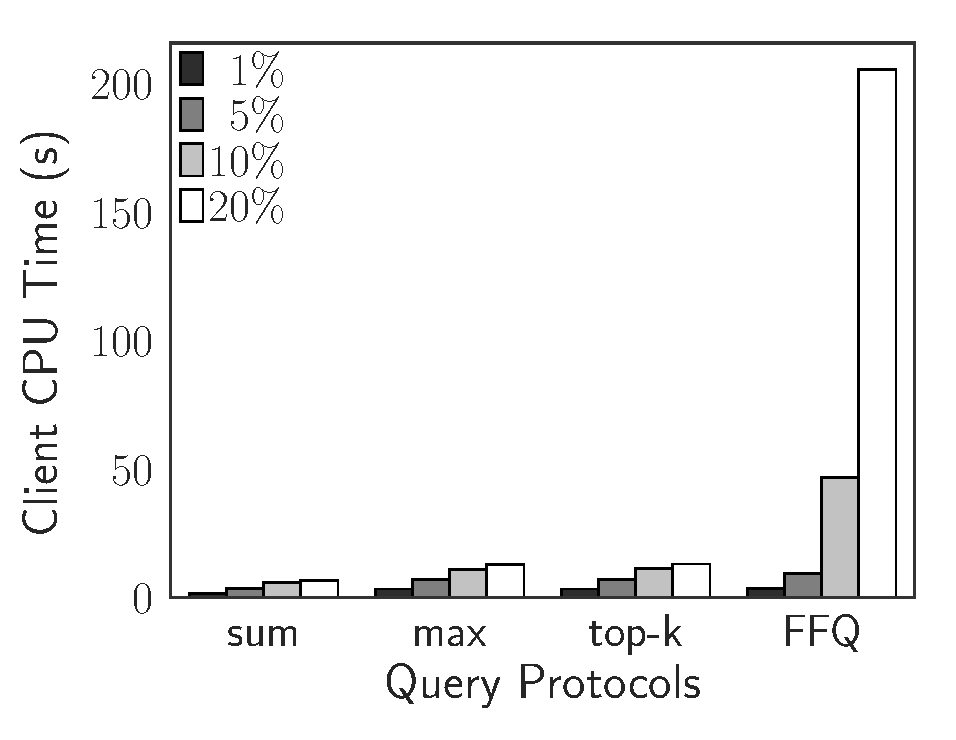
\includegraphics[valign=m,totalheight=\ht\figbox]{exp-figs/aggregate-queries/tpch_client.eps} &
      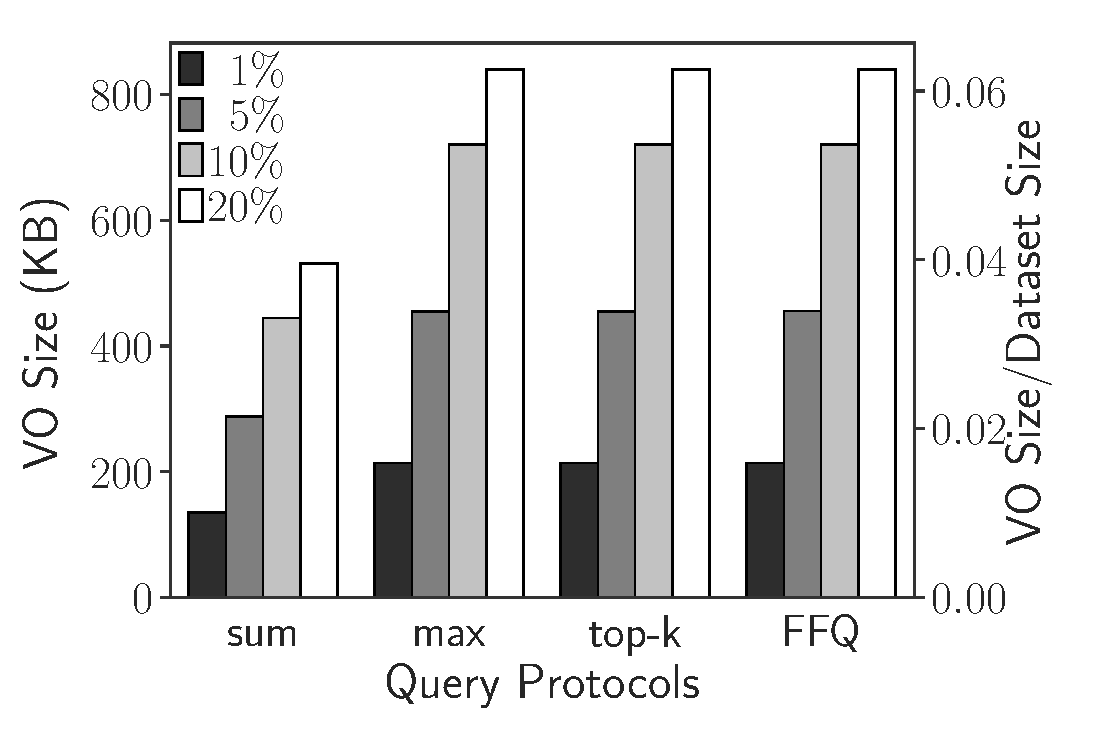
\includegraphics[valign=m,totalheight=\ht\figbox]{exp-figs/aggregate-queries/tpch_vo.eps}
    \end{tabular}
    \caption{Query Performance vs. Selectivity}
  \end{figure}
\end{frame}

\section{Authenticating Relational Queries with Fine-Grained Access Control}

\subsection{Problem Formulation}

\begin{frame}{Problem Model}
  \begin{figure}
    \centering
    \resizebox{.75\linewidth}{!}{\begin{tikzpicture}[remember picture]
  \node (sp) {
      \begin{threeparttable}
        \begin{tabular}{|C|C|C|}
          \hline
          \multicolumn{3}{|c|}{\textbf{Database}} \\ \hline
          q\ attr. & content^{*} & \multicolumn{1}{c|}{access policy} \\ \hline
          o_1      & v_1              & Role_A \land Role_C           \\
          o_2      & v_2              & Role_A \land Role_B           \\
          o_3      & v_3              & Role_B \lor  Role_C           \\
          o_4      & v_4              & Role_C                        \\
          o_5      & v_5              & Role_A                        \\ \hline
        \end{tabular}
        \begin{tablenotes} \footnotesize
        \item[] \hspace{-0.2in} *Content is encrypted by CP-ABE
        \end{tablenotes}
      \end{threeparttable}
    };
  \node[below=0cm of sp] (sp-label) {\textbf{Service Provider (SP)}};

  \draw [Red,rounded corners,thick]
    let \p1 = (sp.west),
    \p2 = ($(sp.south)!.26!(sp.north)$),
    \p3 = ($(sp.west)!.58!(sp.east)$),
    \p4 = ($(sp.south)!.59!(sp.north)$) in
    (\x1, \y2) rectangle (\x3, \y4)
    node[xshift=-0.32cm, yshift=-0.3cm] {$Q$};

  \node[matrix, left=-0.25cm of sp] {
      \node[scale=0.5] at (0,0) (do)
        {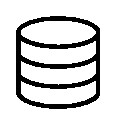
\includegraphics{figs/icons/database.eps}};
      \draw[-latex] (0,0) -- (1.8,0)
        node [above,midway,font=\footnotesize]
        {$\{(o_i, v_i, \Upsilon_i)\}$}
        node [below,midway,font=\footnotesize]
        {$ADS$};
      \\
    };
  \node[xshift=0.5cm] at (sp-label -| do) {\textbf{Data Owner (DO)}};

  \node[matrix, right=-0.25cm of sp] (users) {
      \node[scale=0.9] at (0,0) (user1) {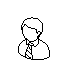
\includegraphics{figs/icons/user.eps}};
      \node[below=0.1cm of user1,font=\footnotesize]{$Role_A, Role_B$};
      \node[right=0cm of user1]{$u_1$};

      \node[scale=0.9] at (0,-2) (user2) {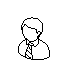
\includegraphics{figs/icons/user.eps}};
      \node[below=0.1cm of user2,font=\footnotesize]{$Role_C$};
      \node[right=0cm of user2]{$u_2$};

      \draw[-latex,transform canvas={yshift=0.5ex}] (0, 0) -- (-2.8, 0)
        node [above,midway,font=\small] {\textcolor{Red}{$Q$}};
        \draw[-latex,transform canvas={yshift=-0.5ex}] (-2.8, 0) -- (0, 0)
        node [below,midway,font=\footnotesize,align=center] {$\{\langle o_2, v_2\rangle , \langle o_3, v_3\rangle\}$ \\ $VO$};

        \draw[-latex,transform canvas={yshift=0.5ex}] (0, -2) -- (-2.8, -2)
        node [above,midway,font=\footnotesize] {\textcolor{Red}{$Q$}};
        \draw[-latex,transform canvas={yshift=-0.5ex}] (-2.8, -2) -- (0, -2)
        node [below,midway,font=\footnotesize,align=center] {$\{\langle o_3, v_3\rangle , \langle o_4, v_4\rangle\}$ \\ $VO$};
        \\
      };
      \node at (sp-label -| user1) (user-label) {\textbf{Clients}};
    \end{tikzpicture}
}
    \caption{Query Authentication with Access Control}
  \end{figure}

  \begin{itemize}[<+->]
    \item \textbf{Problem}
      \begin{itemize}[<1->]
        \item Enforcing \alert{fine-grained access control} to enable big data sharing
        \item Support \alert{equality query}, \alert{range query}, and \alert{join query}
      \end{itemize}
    \item \textbf{Threat Model}
      \begin{itemize}[<1->]
        \item \alert{Integrity}: SP should prove the \emph{soundess} and \emph{completeness} of the results
        \item \alert{Zero-Knowledge Confidentiality}: VO should leak no information beyond query results
      \end{itemize}
  \end{itemize}
\end{frame}

\subsection{Solutions}

\begin{frame}{Equality Query}
  \begin{figure}
    \resizebox{.9\linewidth}{!}{\begin{tikzpicture}[remember picture]
  \node [scale=1] (user) {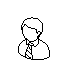
\includegraphics{figs/icons/user.eps}};
  \node [scale=0.6,right=2cm of user](sp){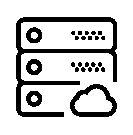
\includegraphics{./figs/icons/server.eps}};
  \onslide<2->{
    \node [matrix, right=2cm of sp] (cases) {
      \onslide<2->{ \node at (0, 1) (case1) {CASE 1: Access Granted $\Upsilon(\mathcal{A}) = 1$}; }
      \onslide<3->{ \node at (0, 0) (case2) {CASE 2: Access Denied $\Upsilon(\mathcal{A}) = 0$}; }
      \onslide<4->{ \node at (0, -1) (case3) {CASE 3: \subnode{case3-inner}{No Record 
\includegraphics[height=2ex]{./figs/icons/warning.eps}}}; }
      \\
    };
  }

  \onslide<4->{
    \node[draw=Red, rectangle callout,
    callout relative pointer={(-1cm, 0)}, right=1cm of case3](warning)
    {\textcolor{Red}{Leak information!}};
  }

  \onslide<5->{
    \node[below=0.3cm of case3-inner.south west, anchor=west]
    {Access Denied $\Upsilon'(\mathcal{A}) = 0$};

    \draw[Red, line width=1pt] ($(case3-inner.west) - (0.1cm, 0)$) -- ($(warning.east) + (0.1cm, 0)$);
  }

  \draw[-latex] (user.east) -- (sp.west) node [above, midway, color=Red] {$Q: \langle o_q, \mathcal{A} \rangle$};

  \onslide<3->{
    \draw[-latex, dashed] (sp.east) -- (case2.west)
    node [midway, scale=1.5, color=Red] (case2-res) {\ding{55}};
  }

  \onslide<2->{
    \draw[-latex] (sp.north) |- (case1.west);
    \node[scale=1.5, color=Green] at (case2-res |- case1.west) {\ding{51}};
  }

  \onslide<4->{
    \draw[-latex, dashed] (sp.south) |- (case3.west);
    \node[scale=1.5, color=Red] at (case2-res |- case3.west) {\ding{55}};
  }

  \onslide<2->{ \node [below=.5cm of cases.south](cases-label){\textbf{Outcomes}}; }
  \node at (user |- cases-label) {\textbf{Client}};
  \node at (sp |- cases-label) {\textbf{Service Provider}};
\end{tikzpicture}
}
    \caption{Equality Query}
  \end{figure}
  \begin{itemize}
    \item<1-> User submits a query key $o_q$ and a role set $\mathcal{A}$
    \item<4-> \myst<5>{\alert{Non-existent record will leak information}}
    \item<5-> Treat non-existent records as \alert{inaccessible by anyone} i.e.\ $\Upsilon' = {Role}_{\emptyset}$
  \end{itemize}
\end{frame}

\begin{frame}{ABS with Predicate Relaxation}
  \begin{itemize}
    \item<+-> \textbf{Attribute Based Signature (ABS)} \\
      \small{It signs a message with a monotone boolean function predicate that is satisfied by the attributes obtained from the authority}
      \begin{figure}
        \resizebox{.85\linewidth}{!}{\begin{tikzpicture}
  \node[matrix] (output) {
    \node[scale=0.9] at (0,1) (user1) {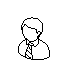
\includegraphics{figs/icons/user.eps}};
    \node[right=0cm of user1] (user1-info) {$u_1$: \textcolor{Green}{Access Granted}};
    \node[scale=0.9] at (0,-1) (user2) {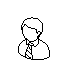
\includegraphics{figs/icons/user.eps}};
    \node[right=-0.1cm of user2] (user2-info) {$u_2$: \textcolor{Red}{Access Denied}};

    \node[below=0cm of user1]{$\Upsilon(\{Role_A, Role_B\}) = 1$};
    \node[below=0cm of user2]{$\Upsilon(\{Role_C\}) = 0$};

    \\
  };

  \coordinate (user-mid) at ($(user1)!.5!(user2)$);

  \node[scale=0.6, left=7cm of user-mid] (input) {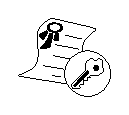
\includegraphics{figs/icons/cert.eps}};
  \node[below=0cm of input, align=center]{
    $\Upsilon = {Role}_A \land {Role}_B$ \\
    $\sigma = \textsf{ABS.Sign}({sk}_\mathcal{A}, m, {Role}_A \land {Role}_B)$
  };

  \coordinate (mid) at ($(input)!.5!(user-mid)$);
  \draw (input.east) -- (mid);
  \draw[-latex] (mid) |- (user1.west);
  \draw[-latex] (mid) |- (user2.west) node[pos=0.75, sloped, scale=2, color=Red] {\ding{55}};

  \node[draw=Red, rectangle callout,
  callout relative pointer={(-1cm, 0)}, right=1cm of user2-info.east](warning)
  {\textcolor{Red}{Leak policy information!}};
\end{tikzpicture}
}
      \end{figure}
    \item<+-> \textbf{Predicate Relaxation} \\
      \small{Derive a \alert{weaker} ABS signature without knowing secret key}
      \begin{figure}
        \resizebox{.85\linewidth}{!}{\begin{tikzpicture}[remember picture]
  \node[matrix] (output) {
    \node[scale=0.6] at (0, -1) (cert1) {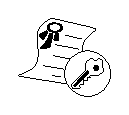
\includegraphics{figs/icons/cert.eps}};
    \node[below=0cm of cert1, align=center]{
      $\Upsilon' = {Role}_C \lor {Role}_\emptyset$ \\
      $\sigma' = \textsf{ABS.Sign}({sk}_\mathcal{A}, m, {Role}_C \lor {Role}_\emptyset)$
    };
    \node[scale=0.6] at (0, 1) (cert2) {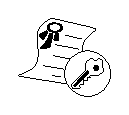
\includegraphics{figs/icons/cert.eps}};
    \node[below=0cm of cert2, align=center]{
      $\Upsilon' = {Role}_A \lor {Role}_B \lor {Role}_\emptyset$ \\
      $\sigma' = \textsf{ABS.Sign}({sk}_\mathcal{A}, m, {Role}_A \lor {Role}_B \lor {Role}_\emptyset)$
    };

    \node[scale=0.9, right=4cm of cert1] (user1) {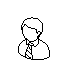
\includegraphics{figs/icons/user.eps}};
    \node[right=0cm of user1] (u1) {$u_1$};
    \node[below=0cm of user1, align=center] {
    $\Upsilon(\{{Role}_A, {Role}_B\})= 1$ \\ $\Upsilon'(\{{Role}_A, {Role}_B\}) = 0$};
    \node[scale=0.9, right=4cm of cert2] (user2) {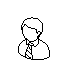
\includegraphics{figs/icons/user.eps}};
    \node[right=0cm of user2]  (u2) {$u_2$: \subnode{u2-inner}{\textcolor{Red}{Access Denied}}};
    \node[below=0cm of user2, align=center] {
    $\Upsilon(\{{Role}_C\})= 0$ \\ $\Upsilon'(\{{Role}_C\}) = 0$};
    \\
  };

  \coordinate (cert-mid) at ($(cert1)!.5!(cert2)$);

  \node[scale=0.6, left=6cm of cert-mid] (input) {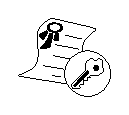
\includegraphics{figs/icons/cert.eps}};
  \node[below=0cm of input, align=center]{
    $\Upsilon = {Role}_A \land {Role}_B$ \\
    $\sigma = \textsf{ABS.Sign}({sk}_\mathcal{A}, m, {Role}_A \land {Role}_B)$
  };

  \coordinate (mid) at ($(input)!.45!(cert-mid)$);
  \draw (input.east) -- (mid);
  \draw[-latex] (mid) |- (cert1.west) node[pos=0.75, sloped] {X};
  \draw[-latex] (mid) |- (cert2.west) node[pos=0.75, sloped, scale=2, color=Green] {\ding{51}};

  \node[draw=Green, rectangle callout,
  callout absolute pointer={(u2-inner.south)}, below=0.1cm of u2-inner.south, xshift=0.3cm]
  {\textcolor{Green}{No policy leak!}};
\end{tikzpicture}
}
      \end{figure}
  \end{itemize}
\end{frame}

\begin{frame}{Authenticated Data Structures}
  \setbeamerfont{block title example}{size=\small}
  \setbeamerfont{block body example}{size=\small}
  \begin{itemize}
    \item<+-> \emph{Access-Policy-Preserving} (APP) signature
      \begin{itemize}
        \item Signed by DO and used as \alert{ADS}
        \item It captures three parts of information: \alert{query attribute $o_i$}, \alert{data content $v_i$}, and \alert{access policy $\Upsilon_i$}
      \end{itemize}
      \begin{example}
        \begin{align*}
         & \text{Record}_2 \gets \langle o_2, v_2, \Upsilon_2 = {Role}_A \land {Role}_B \rangle                  \\
         & \sigma_2 \gets \textsf{ABS.Sign}({sk}_{\textrm{DO}}, hash(o_2) | hash(v_2) , {Role}_A \land {Role}_B)
        \end{align*}
      \end{example}
    \item<+-> \emph{Access-Policy-Stripped} (APS) signature
      \begin{itemize}
        \item Replace $\Upsilon_i$ to \alert{$\hat{\Upsilon}_{\mathcal{A}} = a_1 \lor a_2 \lor \dots \lor a_n, a_i \in \mathbb{A}\backslash\mathcal{A}$}
        \item Be used to prove inaccessibility in \alert{zero-knowledge}
      \end{itemize}
      \begin{example}
        \begin{align*}
         & \mathbb{A} = \{ {Role}_A, {Role}_B, {Role}_C, {Role}_\emptyset \},
         \hat{\Upsilon}_{\{{Role}_C\}} = {Role}_A \lor {Role}_B \lor {Role}_\emptyset
         \\
         & \hat{\sigma}_2 \gets \textsf{ABS.Sign}({sk}_{\textrm{DO}}, hash(o_2) | hash(v_2) , {Role}_A \lor {Role}_B \lor {Role}_\emptyset)
        \end{align*}
      \end{example}
  \end{itemize}
\end{frame}

\begin{frame}{Query Processing}
  \begin{figure}
    \footnotesize
    \resizebox{.8\linewidth}{!}{\begin{tikzpicture}
  \node[matrix] (users) {
    \onslide<2->{
      \node[scale=0.9] at (0,0) (user1) {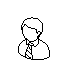
\includegraphics{figs/icons/user.eps}};
      \node[below=0cm of user1]{$Role_A, Role_B$};
      \node[right=0cm of user1]{$u_1$};
    }
    \onslide<4->{
      \node[scale=0.9] at (0,-1.5) (user2) {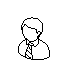
\includegraphics{figs/icons/user.eps}};
      \node[below=-0.1cm of user2]{$Role_C$};
      \node[right=-0.1cm of user2]{$u_2$};
    }
    \\
  };

  \coordinate (user_mid) at ($(user1)!.5!(user2)$);

  \onslide<5->{
    \node (aps) [left=3.2cm of user2,align=center] {APS signature\\$\hat{\sigma}_{2, \mathcal{A}_{u_2}}$};
    \node [draw,thick,fit=(aps),rounded corners] (aps_round) {};
  }

  \onslide<1->{
    \node (app) [left=5.2cm of user1,align=center] {APP signature\\$\sigma_2$};
    \node [draw,thick,fit=(app),rounded corners] (app_round) {};
  }

  \onslide<1->{
    \node (data) [left=8cm of user2,align=center]
    {$\langle o_2, v_2, \Upsilon_2\rangle$\\$\Upsilon_2 = Role_A \land Role_B$};
    \node [draw,thick,fit=(data),rounded corners] (data_round) {};
  }

  \draw<3->[-latex, thick] (app_round.east) -- ($(user1) - (0.5cm, 0)$)
  node [above,midway] (vo1) {};
  \onslide+<5->{
    \draw[-latex, thick] (aps_round.east) -- ($(user2) - (0.5cm, 0)$)
    node [above,midway] (vo2) {$\langle hash(v_2), \hat{\sigma}_{2, \mathcal{A}_{u_2}}\rangle$};
  }
  \draw<3-> (vo2 |- vo1) node [above] {$\langle v_2, \sigma_2, \Upsilon_2\rangle$};

  \draw<5->[-latex, thick] (app_round.south) .. controls (app_round.south |- aps_round.west)
  .. (aps_round.west)
  node[below,midway,pos=0.55,xshift=-0.3cm,yshift=-0.1cm] {\textsf{ABS.Relax}};

  \draw<1->[-latex, thick] (data_round.north) .. controls (data_round.north |- app_round.west)
  .. (app_round.west)
  node[above,midway,pos=0.75] {\textsf{ABS.Sign}};

  \coordinate (do_sp_mid) at ($(data_round.east)!.5!(app_round.west)$);
  \draw[dashed, color=black!30] ($(do_sp_mid) - (0,1.8cm)$) -- ($(do_sp_mid) + (0,1.5cm)$);

  \coordinate (sp_user_mid_x) at ($(aps_round.east) + (0.1cm, 0)$);
  \coordinate (sp_user_mid) at (do_sp_mid -| sp_user_mid_x);
  \draw[dashed, color=black!30] ($(sp_user_mid) - (0,1.8cm)$) -- ($(sp_user_mid) + (0,1.5cm)$);

  \node[below=0.15cm of data_round.south] (do-label) {\textbf{Data Owner (DO)}};
  \draw let \p1 = ($(sp_user_mid)!0.5!(do_sp_mid)$), \p2 = (do-label) in (\x1, \y2)
  node {\textbf{Service Provider (SP)}};
  \node<2-> at (do-label -| user1) (user-label) {\textbf{Users}};
\end{tikzpicture}
}
    \caption{Equality Query Authentication}
  \end{figure}
  \begin{itemize}
    \item<1-> DO generates ADS and sends to the SP
    \item<2-> $u_1$ \alert{can access the data}, \onslide<3->{APP signature is the VO}
    \item<4-> $u_2$ \alert{cannot access the data},
      \onslide<5->{SP generates an \textcolor{Red}{APS signature} as VO}
  \end{itemize}
\end{frame}

\begin{frame}{Range Query Authentication}
  \begin{figure}
    \begin{subfigure}[b]{.5\linewidth}
      \centering
      \resizebox{\linewidth}{!}{\begin{minipage}[t]{.6\linewidth}
  \resizebox{\linewidth}{!}{%
    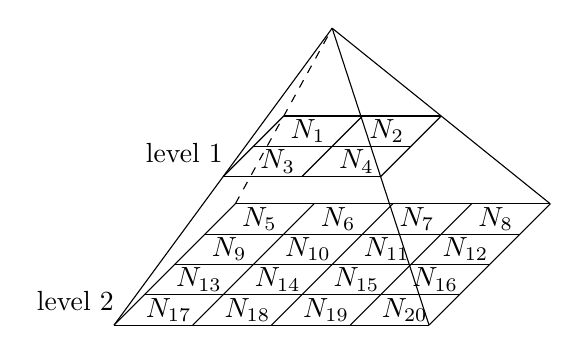
\begin{tikzpicture}
      % level 1
      \node at (-1.8, 1.5, 0.2) {level 1};
      \foreach \x [count=\xi] in {-0.5, 0.5}{
        \foreach \z [count=\zi] in {-0.5, 0.5}{
          \pgfmathtruncatemacro{\i}{\zi*2 + \xi - 2};
          \node at(\x, 1.5, \z) {$N_{\i}$};
        }
      }
      \foreach \x in {-1,...,1}{\draw (\x,1.5,-1) -- (\x,1.5,1);}
      \foreach \z in {-1,...,1}{\draw (-1,1.5,\z) -- (1,1.5,\z);}
      % level 2
      \node at (-2.8, 0, 1.2) {level 2};
      \foreach \x [count=\xi] in {-1.5,-0.5,...,1.5}{
        \foreach \z [count=\zi] in {-1.5,-0.5,...,1.5}{
          \pgfmathtruncatemacro{\i}{\zi*4 + \xi};
          \node at(\x, 0, \z) {$N_{\i}$};
        }
      }
      \foreach \x in {-2,...,2}{\draw (\x,0,-2) -- (\x,0,2);}
      \foreach \z in {-2,...,2}{\draw (-2,0,\z) -- (2,0,\z);}
      % pyramid
      \draw (-2,0,2) -- (0,3,0);
      \draw (2,0,2) -- (0,3,0);
      \draw (2,0,-2) -- (0,3,0);
      \draw[dashed] (-2,0,-2) -- (0,3,0);
    \end{tikzpicture}
  }
\end{minipage}~%
\begin{minipage}[t]{.3\linewidth}
  \resizebox{\linewidth}{!}{%
    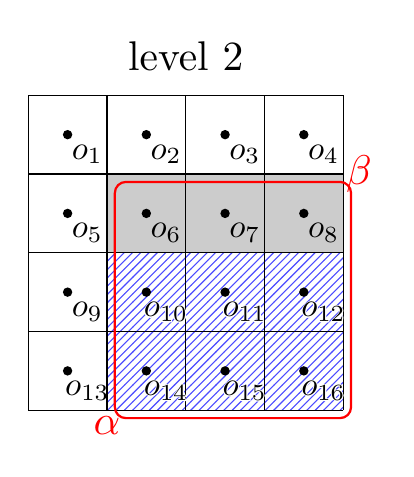
\begin{tikzpicture}
      \node[scale=1.5] at (0, 2.5) {level 2};
      \foreach \x in {-2,...,2}{\draw (\x,-2) -- (\x,2);}
      \foreach \y in {-2,...,2}{\draw (-2,\y) -- (2,\y);}
      \foreach \y [count=\yi] in {1.5,0.5,...,-1.5}{%
        \foreach \x [count=\xi] in {-1.5,-0.5,...,1.5}{%
          \pgfmathtruncatemacro{\i}{\yi*4 + \xi - 4};
          \node [circle,fill,inner sep=1.2pt] at (\x,\y) {};
          \ifthenelse{\i=10 \OR \i=11 \OR \i=12 \OR \i=14 \OR \i=15 \OR \i=16}{
            \node[scale=1.2] at (\x+0.25,\y-0.25) {\contour{white}{$o_{\i}$}};
            }{
            \node[scale=1.2] at (\x+0.25,\y-0.25) {$o_{\i}$};
          }
        }
      }
      \draw[Red,rounded corners,thick] (-0.9,-2.1) rectangle (2.1,0.9);
      \node[Red,scale=1.5] at (-1,-2.2) {$\alpha$};
      \node[Red,scale=1.5] at (2.2,1) {$\beta$};
      \begin{pgfonlayer}{background}
        \fill[color=black!20] (-1,0) rectangle (2,1);
        \fill[pattern=north east lines,pattern color=blue!70] (-1,-2) rectangle (2,0);
      \end{pgfonlayer}
    \end{tikzpicture}
  }
\end{minipage}
}
      \caption{Structure}
    \end{subfigure}~%
    \begin{subfigure}[b]{.5\linewidth}
      \centering
      \resizebox{\linewidth}{!}{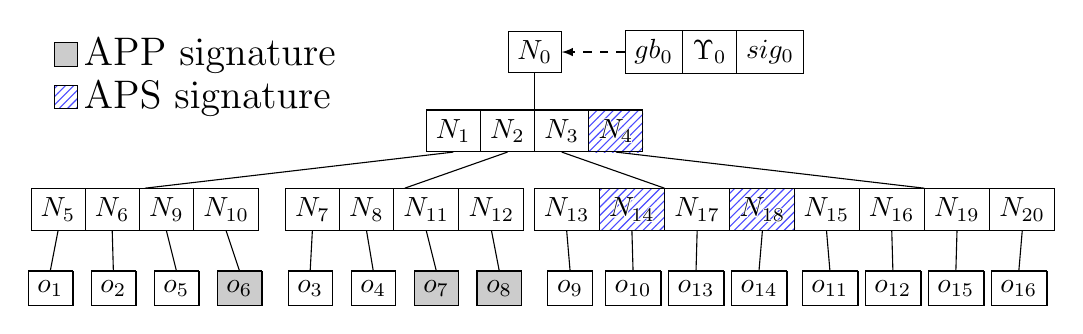
\begin{tikzpicture}
  \tikzstyle{tree node}=[
  rectangle split,
  rectangle split horizontal,
  rectangle split ignore empty parts,
  draw
  ]
  \tikzstyle{tree}=[
  every node/.style={tree node},
  edge from parent path={},
  level/.style={level distance=1cm},
  level 2/.style={sibling distance=3.3cm},
  level 3/.style={sibling distance=0.8cm},
  ]

  \path[tree] node (root) {$N_0$}
  child {
    node (l1) {
      \nodepart{one} $N_1$ \nodepart{two} $N_2$
      \nodepart{three} $N_3$ \nodepart{four} \contour{white}{$N_4$}
    }
    child {
      node (l21) {
        \nodepart{one} $N_{5}$ \nodepart{two} $N_{6}$
        \nodepart{three} $N_{9}$ \nodepart{four} $N_{10}$
      }
      child {node (o1) {$o_1$}}
      child {node (o2) {$o_2$}}
      child {node (o5) {$o_5$}}
      child {node [fill=black!20, text=black] (o6) {$o_6$}}
    }
    child {
      node (l22) {
        \nodepart{one} $N_{7}$ \nodepart{two} $N_{8}$
        \nodepart{three} $N_{11}$ \nodepart{four} $N_{12}$
      }
      child {node (o3) {$o_3$}}
      child {node (o4) {$o_4$}}
      child {node (o7) [fill=black!20, text=black] {$o_7$}}
      child {node (o8) [fill=black!20, text=black] {$o_8$}}
    }
    child {
      node (l23) {
        \nodepart{one} $N_{13}$ \nodepart{two} \contour{white}{$N_{14}$}
        \nodepart{three} $N_{17}$ \nodepart{four} \contour{white}{$N_{18}$}
      }
      child {node (o9) {$o_9$}}
      child {node (o10) {$o_{10}$}}
      child {node (o13) {$o_{13}$}}
      child {node (o14) {$o_{14}$}}
    }
    child {
      node (l24) {
        \nodepart{one} $N_{15}$ \nodepart{two} $N_{16}$
        \nodepart{three} $N_{19}$ \nodepart{four} $N_{20}$
      }
      child {node (o11) {$o_{11}$}}
      child {node (o12) {$o_{12}$}}
      child {node (o15) {$o_{15}$}}
      child {node (o16) {$o_{16}$}}
    }
  };

  \begin{pgfonlayer}{background}
    \fill[pattern=north east lines,pattern color=blue!70] (l1.three split north) rectangle (l1.south east);
    \fill[pattern=north east lines,pattern color=blue!70] (l23.one split north) rectangle (l23.two split south);
    \fill[pattern=north east lines,pattern color=blue!70] (l23.three split north) rectangle (l23.south east);
  \end{pgfonlayer}

  \foreach \a/\b in {
    root.south/l1,
    l1.one south/l21,
    l1.two south/l22,
    l1.three south/l23,
    l1.four south/l24,
    l21.one south/o1,
    l21.two south/o2,
    l21.three south/o5,
    l21.four south/o6,
    l22.one south/o3,
    l22.two south/o4,
    l22.three south/o7,
    l22.four south/o8,
    l23.one south/o9,
    l23.two south/o10,
    l23.three south/o13,
    l23.four south/o14,
    l24.one south/o11,
    l24.two south/o12,
    l24.three south/o15,
    l24.four south/o16%
  }
  \draw [style=edge from parent] (\a) -- (\b.north);

  \node[tree node,right=0.8cm of root] (data)
  {$gb_0$ \nodepart{two} $\Upsilon_0$ \nodepart{three} $sig_0$};

  \draw[dashed,-latex] (data) -- (root);

  \begin{customlegend}[
    legend cell align=left,
    legend image code/.code={%
      \draw[#1] (0cm,-0.15cm) rectangle (0.3cm,0.15cm);
    },
    legend style={draw=none,left=2cm of root,yshift=-0.3cm,font={\Large}}
    ]
    \addlegendimage{black,fill=black!20}
    \addlegendentry{APP signature}
    \addlegendimage{black,pattern=north east lines,pattern color=blue!70}
    \addlegendentry{APS signature}
  \end{customlegend}
\end{tikzpicture}
}
      \caption{Index}
    \end{subfigure}
    \caption{Access-Policy-Preserving Grid-Tree (AP$^2$G-Tree)}
  \end{figure}

  \begin{itemize}
    \item \alert{Non-Leaf Node} $p_i = p_{c_1}  \lor  p_{c_2}  \lor  \dots  \lor  p_{c_C}$, $sig_i = \textsf{ABS.Sign}({sk}_{\textrm{DO}}, gb_i , p_i)$
    \item \alert{Leaf Node} Identical to those of underlying record
  \end{itemize}
\end{frame}

\begin{frame}{Join Query Authentication}
  \begin{figure}
    \centering
    \resizebox{.65\linewidth}{!}{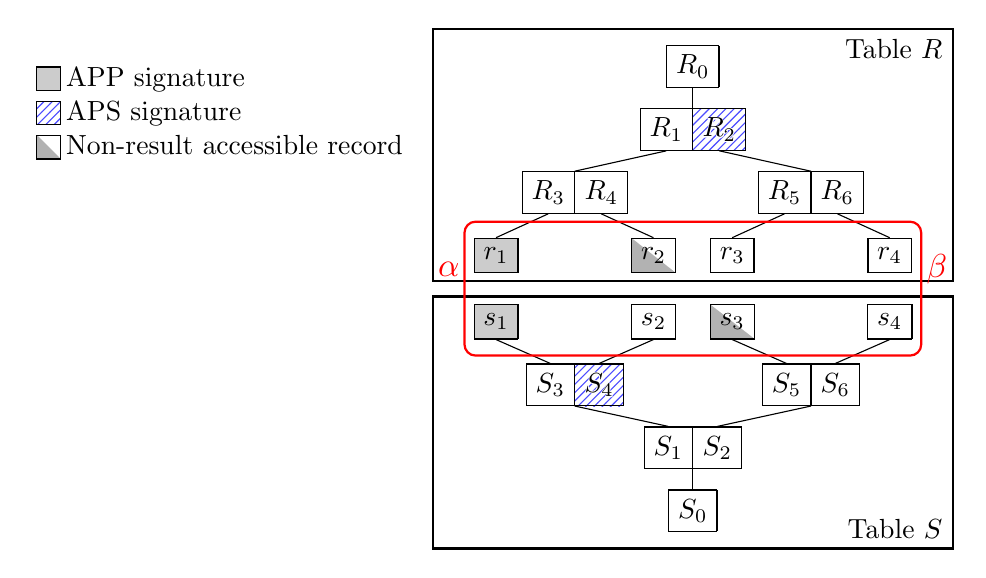
\begin{tikzpicture}
  \tikzstyle{tree node}=[
  rectangle split,
  rectangle split horizontal,
  rectangle split ignore empty parts,
  draw
  ]
  \tikzstyle{tree}=[
  every node/.style={tree node},
  edge from parent path={},
  level/.style={level distance=0.8cm},
  level 2/.style={sibling distance=3cm},
  level 3/.style={sibling distance=2cm},
  ]
  \tikzstyle{diagonal fill}=[
  path picture={
    \fill[#1] (path picture bounding box.north west) |-
    (path picture bounding box.south east) -- cycle;
  }
  ]

  \path[tree] node (r_root) {$R_0$}
  child {
    node (r_l1) {
      \nodepart{one} $R_1$ \nodepart{two} \contour{white}{$R_2$}
    }
    child {
      node (r_l21) {
        \nodepart{one} $R_{3}$ \nodepart{two} $R_{4}$
      }
      child {node (r1) [fill=black!20, text=black] {$r_1$}}
      child {node (r2) [diagonal fill=black!30, text=black] {$r_2$}}
    }
    child {
      node (r_l22) {
        \nodepart{one} $R_{5}$ \nodepart{two} $R_{6}$
      }
      child {node (r3) {$r_3$}}
      child {node (r4) {$r_4$}}
    }
  };

  \path[tree, grow=up] node[below=5.1cm of r_root] (s_root) {$S_0$}
  child {
    node (s_l1) {
      \nodepart{one} $S_1$ \nodepart{two} $S_2$
    }
    child {
      node (s_l22) {
        \nodepart{one} $S_{5}$ \nodepart{two} $S_{6}$
      }
      child {node (s4) {$s_4$}}
      child {node (s3) [diagonal fill=black!30, text=black] {$s_3$}}
    }
    child {
      node (s_l21) {
        \nodepart{one} $S_{3}$ \nodepart{two} \contour{white}{$S_{4}$}
      }
      child {node (s2) {$s_2$}}
      child {node (s1) [fill=black!20, text=black] {$s_1$}}
    }
  };

  \begin{pgfonlayer}{background}
    \fill[pattern=north east lines,pattern color=blue!70] (r_l1.one split north) rectangle (r_l1.south east);
    \fill[pattern=north east lines,pattern color=blue!70] (s_l21.one split north) rectangle (s_l21.south east);
  \end{pgfonlayer}

  \foreach \a/\b in {
    r_root.south/r_l1,
    r_l1.one south/r_l21,
    r_l1.two south/r_l22,
    r_l21.one south/r1,
    r_l21.two south/r2,
    r_l22.one south/r3,
    r_l22.two south/r4%
  }
  \draw [style=edge from parent] (\a) -- (\b.north);
  \foreach \a/\b in {
    s_root.north/s_l1,
    s_l1.one north/s_l21,
    s_l1.two north/s_l22,
    s_l21.one north/s1,
    s_l21.two north/s2,
    s_l22.one north/s3,
    s_l22.two north/s4%
  }
  \draw [style=edge from parent] (\a) -- (\b.south);

  \coordinate (mid) at ($(r_root)!.5!(s_root)$);

  \draw[thick] ($(mid) + (-3.3cm,0.1cm)$) rectangle
  ($(mid) + (3.3cm,3.3cm)$) node[anchor=north east,scale=1] {Table $R$};

  \draw[thick] ($(mid) + (-3.3cm,-0.1cm)$) rectangle
  ($(mid) + (3.3cm,-3.3cm)$) node[anchor=south east,scale=1] {Table $S$};

  \draw[Red, rounded corners, thick]
  ($(mid) - (2.9cm,0.85cm)$) rectangle ($(mid) + (2.9cm,0.85cm)$);
  \node[Red,scale=1.2] at ($(mid) + (-3.1cm,0.25cm)$) {$\alpha$};
  \node[Red,scale=1.2] at ($(mid) + ( 3.1cm,0.25cm)$) {$\beta$};

  \begin{customlegend}[
    legend cell align=left,
    rectangle legend/.style={
      legend image code/.code={%
        \draw[black,#1] (0cm,-0.15cm) rectangle (0.3cm,0.15cm);
      }
    },
    rectangle legend multiline/.style={
      legend image code/.code={%
        \draw[black,#1] (0cm,-0.15cm) rectangle (0.3cm,0.15cm);
      }
    },
    legend style={
      draw=none,
      cells={align=left},
      above left=1.5cm and 3.5cm of mid
    }
    ]
    \addlegendimage{rectangle legend={fill=black!20}}
    \addlegendentry{APP signature}
    \addlegendimage{rectangle legend={pattern=north east lines,pattern color=blue!70}}
    \addlegendentry{APS signature}
    \addlegendimage{rectangle legend multiline={diagonal fill=black!30}}
    \addlegendentry{Non-result accessible record}
  \end{customlegend}
\end{tikzpicture}
}
    \caption{Join Query Authentication}
  \end{figure}

  \begin{itemize}
    \item Use \alert{APP signature} to prove soundness
    \item Use \alert{APS signature} to prove completeness
  \end{itemize}
\end{frame}

\subsection{Performance Evaluation}

\begin{frame}{Performance Evaluation}
  \begin{table}
    \footnotesize
    \centering
    \begin{tabular}{cccc}
      \toprule
      \multirow{2}{*}{\tabincell{c}{Database\\Scale}} &
      \multicolumn{2}{c}{DO CPU Time} &
      \multirow{2}{*}{\tabincell{c}{Index Size (Tree Structure~+~Signatures) \\(GB)}} \\
      \cmidrule(lr){2-3}
                                      &
      Sign APPs (h) & Build Index (h) &
      \\
      \midrule
      0.1  & 0.63 & 0.74 & 2.47 (0.49 + 1.98) \\
      0.3  & 0.77 & 0.95 & 2.93 (0.56 + 2.37) \\
      1    & 0.86 & 1.00 & 3.14 (0.58 + 2.56) \\
      3    & 0.87 & 1.01 & 3.16  (0.59 + 2.57) \\
      \bottomrule
    \end{tabular}
    \caption{DO Setup Overhead}\label{tab:access-control:do-setup}
  \end{table}
  \begin{itemize}
    \item Dataset:
      \begin{itemize}
        \item TPC-H dataset: \\
          0.1 ($\fnum{600000}$ records), \emph{0.3 ($\fnum{1800000}$ records)}, 1 ($\fnum{6000000}$ records), and 3 ($\fnum{18000000}$ records)
        \item $10$ distinct policies ($10$ global roles, max policy length is $6$)
      \end{itemize}
  \end{itemize}
\end{frame}

\begin{frame}{Performance Evaluation}
  \savebox{\figbox}{%
    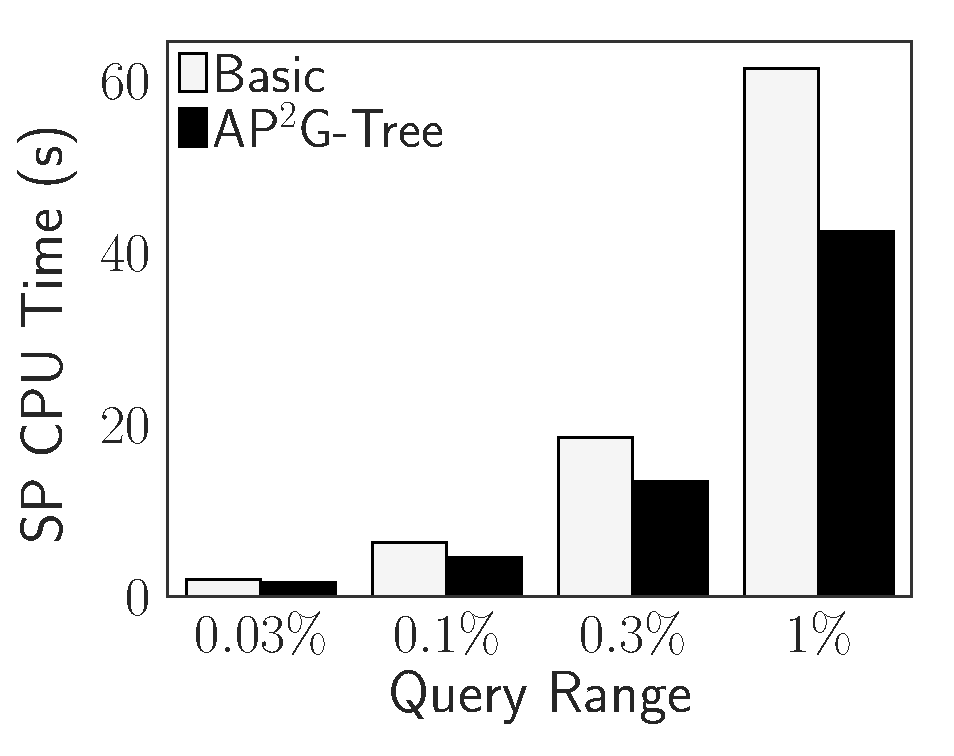
\includegraphics[height=.35\textheight]{exp-figs/access-control/range_sp.eps}%
  }
  \begin{figure}
    \centering
    \begin{subfigure}{.33\linewidth}
      \centering
      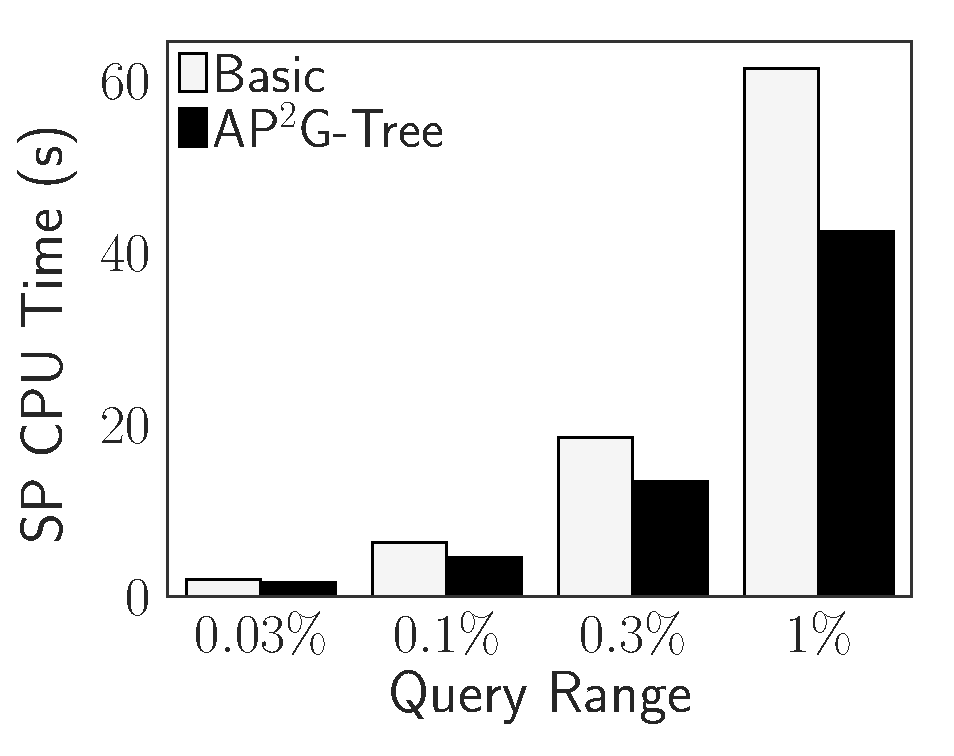
\includegraphics[height=\ht\figbox]{exp-figs/access-control/range_sp.eps}
      \caption{SP CPU Time}
    \end{subfigure}~%
    \begin{subfigure}{.33\linewidth}
      \centering
      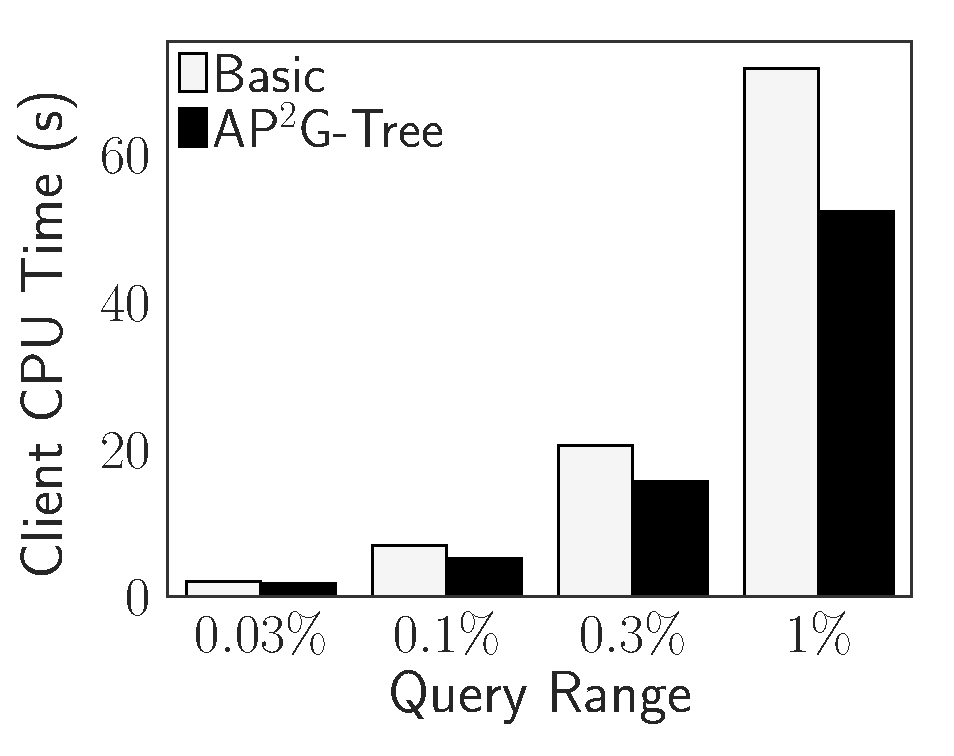
\includegraphics[height=\ht\figbox]{exp-figs/access-control/range_user.eps}
      \caption{Client CPU Time}
    \end{subfigure}~%
    \begin{subfigure}{.33\linewidth}
      \centering
      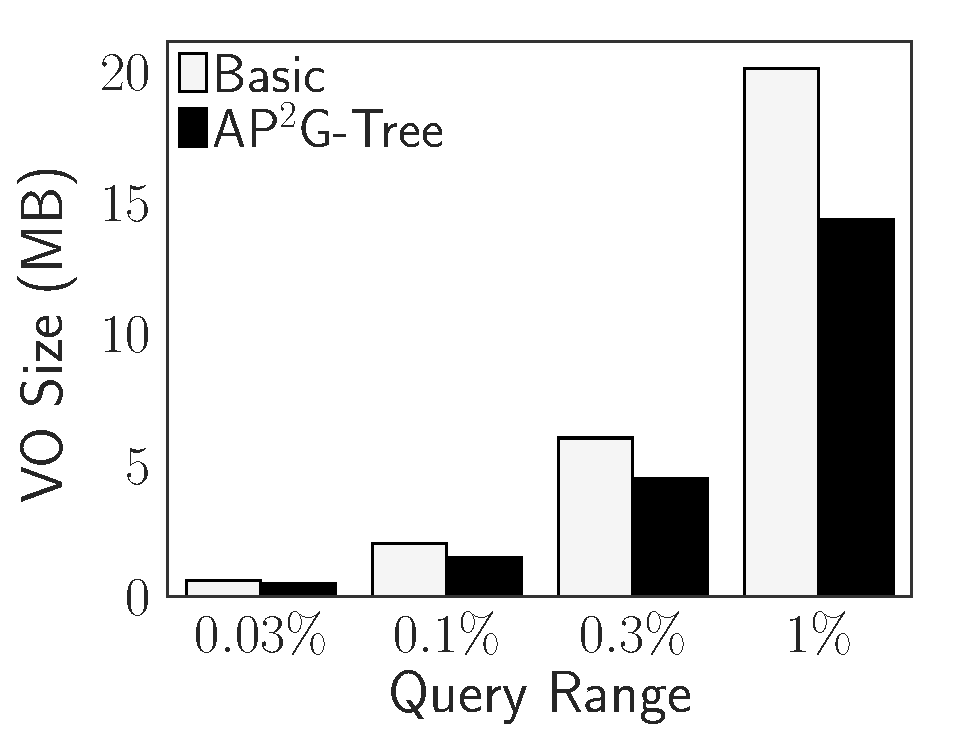
\includegraphics[height=\ht\figbox]{exp-figs/access-control/range_vo.eps}
      \caption{VO Size}
    \end{subfigure}
    \caption{Range Query Performance vs. Range}
  \end{figure}
  \vspace{-3ex}
  \begin{figure}
    \centering
    \begin{subfigure}{.33\linewidth}
      \centering
      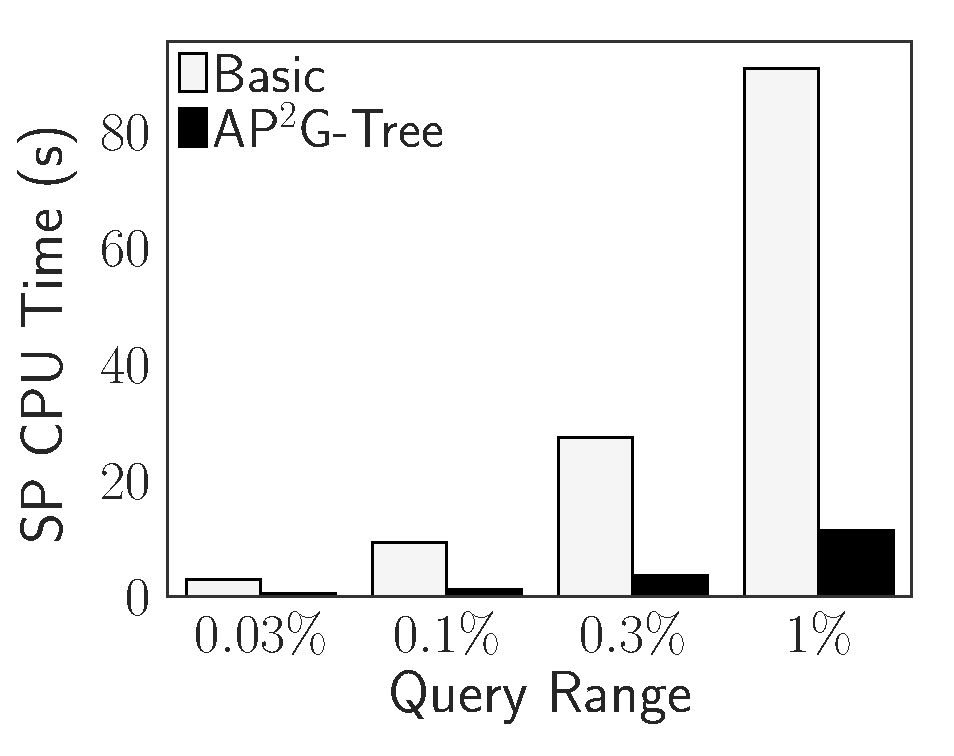
\includegraphics[height=\ht\figbox]{exp-figs/access-control/join_sp.eps}
      \caption{SP CPU Time}
    \end{subfigure}~%
    \begin{subfigure}{.33\linewidth}
      \centering
      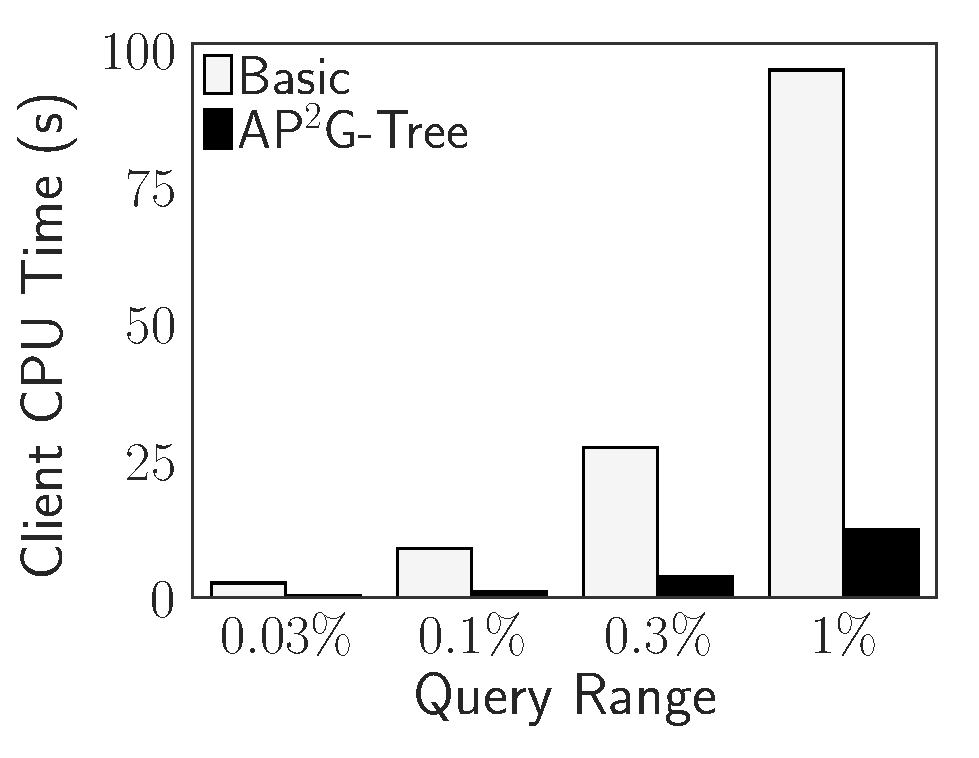
\includegraphics[height=\ht\figbox]{exp-figs/access-control/join_user.eps}
      \caption{Client CPU Time}
    \end{subfigure}~%
    \begin{subfigure}{.33\linewidth}
      \centering
      \includegraphics[height=\ht\figbox]{exp-figs/access-control/join_vo.eps}
      \caption{VO Size}
    \end{subfigure}
    \caption{Join Query Performance vs. Range}
  \end{figure}
\end{frame}

\section{Authenticating {kNN} Queries in Distributed Settings}

\subsection{Problem Formulation}

\subsection{Solutions}

\subsection{Performance Evaluation}

\section{Conclusions}

\begin{frame}{Contributions}
\end{frame}

\begin{frame}{Future Directions}
\end{frame}

\begin{frame}[standout]
  Thanks \\
  Questions?
\end{frame}

\appendix%

\begin{frame}{PA$^2$ on Candidate Object Selection (Optimized)}
  \begin{figure}
    \includegraphics[width=.4\linewidth]{figs/aggregate-queries/grid_tree_opt.eps}
    \caption{Optimized MG-tree}
  \end{figure}
  \metroset{block=transparent}
  \begin{alertblock}{Optimized Digest for Non-Leaf Node}
    \begin{align*}
      dig_i = H(gb_{c_1} | H(acc(S_{c_1})| acc(U_{c_1})) | dig_{c_1} | \dotsb
      |gb_{c_C} | H(acc(S_{c_C})|acc(U_{c_C})) | dig_{c_C})
    \end{align*}
  \end{alertblock}
\end{frame}

\begin{frame}{Optimizations of Authenticating Queries with Fine-Grained Access Control}
  \begin{itemize}[<+->]
    \item \alert{General Optimizations}:
      \begin{itemize}[<1->]
        \item Hierarchical Role Assignment
        \item Parallelism
      \end{itemize}
    \item \alert{Relaxing Zero-Knowledge Requirement}:
      \begin{figure}
        \begin{subfigure}[b]{.5\linewidth}
          \centering
          \resizebox{\linewidth}{!}{\begin{minipage}[t]{.6\linewidth}
  \resizebox{\linewidth}{!}{%
    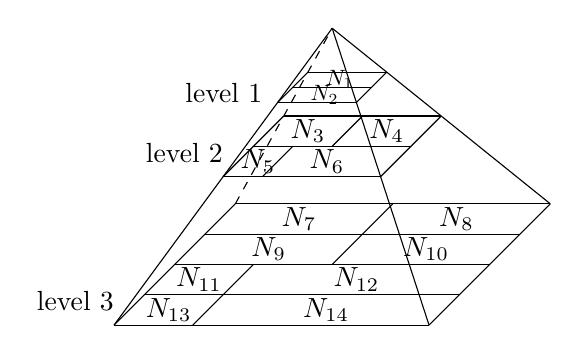
\begin{tikzpicture}
      % level 1
      \node at (-1.3, 2.25, 0.2) {level 1};
      \draw(-0.5,2.25,-0.5) -- (-0.5,2.25,0.5);
      \draw(-0.5,2.25,-0.5) -- (0.5,2.25,-0.5);
      \draw(0.5,2.25,-0.5) -- (0.5,2.25,0.5);
      \draw(-0.5,2.25,0.5) -- (0.5,2.25,0.5);
      \draw(-0.5,2.25,0) -- (0.5,2.25,0);
      \foreach \x/\z [count=\i] in
      {0/-0.25,0/0.25}{
        \node[scale=0.8] at(\x, 2.25, \z) {$N_{\i}$};
      }
      % level 2
      \node at (-1.8, 1.5, 0.2) {level 2};
      \draw (-1,1.5,-1) -- (-1,1.5,1);
      \draw (-1,1.5,-1) -- (1,1.5,-1);
      \draw (1,1.5,-1) -- (1,1.5,1);
      \draw (-1,1.5,1) -- (1,1.5,1);
      \draw (-1,1.5,0) -- (1,1.5,0);
      \draw (0,1.5,-1) -- (0,1.5,0);
      \draw (-0.5,1.5,0) -- (-0.5,1.5,1);
      \foreach \x/\z [count=\i from 3] in
      {-0.5/-0.5,0.5/-0.5,-0.75/0.5,0.125/0.5}{
        \node at(\x, 1.5, \z) {$N_{\i}$};
      }
      % level 3
      \node at (-2.8, 0, 1.2) {level 3};
      \draw (-2,0,-2) -- (-2,0,2);
      \draw (-2,0,-2) -- (2,0,-2);
      \draw (2,0,-2) -- (2,0,2);
      \draw (-2,0,2) -- (2,0,2);
      \draw (-2,0,0) -- (2,0,0);
      \draw (0,0,0) -- (0,0,-2);
      \draw (-1,0,0) -- (-1,0,2);
      \draw (-2,0,1) -- (2,0,1);
      \draw (-2,0,-1) -- (2,0,-1);
      \foreach \x/\z [count=\i from 7] in
      {-1/-1.5,1/-1.5,-1/-0.5,1/-0.5,-1.5/0.5,0.5/0.5,-1.5/1.5,0.5/1.5}{
        \node at(\x, 0, \z) {$N_{\i}$};
      }

      % pyramid
      \draw (-2,0,2) -- (0,3,0);
      \draw (2,0,2) -- (0,3,0);
      \draw (2,0,-2) -- (0,3,0);
      \draw[dashed] (-2,0,-2) -- (0,3,0);
    \end{tikzpicture}
  }
\end{minipage}~%
\begin{minipage}[t]{.3\linewidth}
  \resizebox{\linewidth}{!}{%
    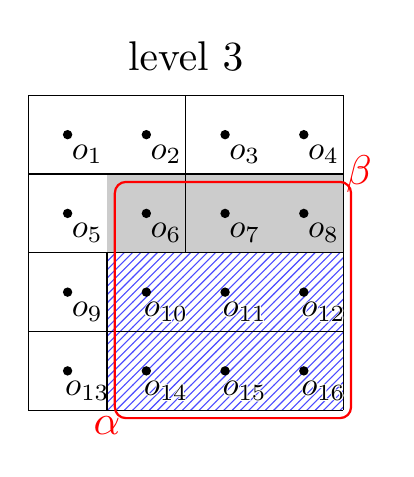
\begin{tikzpicture}
      \node[scale=1.5] at (0, 2.5) {level 3};
      \draw (-2,-2) -- (-2,2);
      \draw (-2,-2) -- (2,-2);
      \draw (2,-2) -- (2,2);
      \draw (-2,2) -- (2,2);

      % level 1
      \draw (-2,0) -- (2,0);
      % level 2
      \draw (0,0) -- (0,2);
      \draw (-1,0) -- (-1,-2);
      % level 3
      \draw (-2,1) -- (2,1);
      \draw (-2,-1) -- (2,-1);

      \foreach \y [count=\yi] in {1.5,0.5,...,-1.5}{%
        \foreach \x [count=\xi] in {-1.5,-0.5,...,1.5}{%
          \pgfmathtruncatemacro{\i}{\yi*4 + \xi - 4};
          \node [circle,fill,inner sep=1.2pt] at (\x,\y) {};
          \ifthenelse{\i=10 \OR \i=11 \OR \i=12 \OR \i=14 \OR \i=15 \OR \i=16}{
            \node[scale=1.2] at (\x+0.25,\y-0.25) {\contour{white}{$o_{\i}$}};
            }{
            \node[scale=1.2] at (\x+0.25,\y-0.25) {$o_{\i}$};
          }
        }
      }
      \draw[Red,rounded corners,thick] (-0.9,-2.1) rectangle (2.1,0.9);
      \node[Red,scale=1.5] at (-1,-2.2) {$\alpha$};
      \node[Red,scale=1.5] at (2.2,1) {$\beta$};
      \begin{pgfonlayer}{background}
        \fill[color=black!20] (-1,0) rectangle (2,1);
        \fill[pattern=north east lines,pattern color=blue!70] (-1,-2) rectangle (2,0);
      \end{pgfonlayer}
    \end{tikzpicture}
  }
\end{minipage}
}
          \caption{Structure}
        \end{subfigure}~%
        \begin{subfigure}[b]{.5\linewidth}
          \centering
          \resizebox{\linewidth}{!}{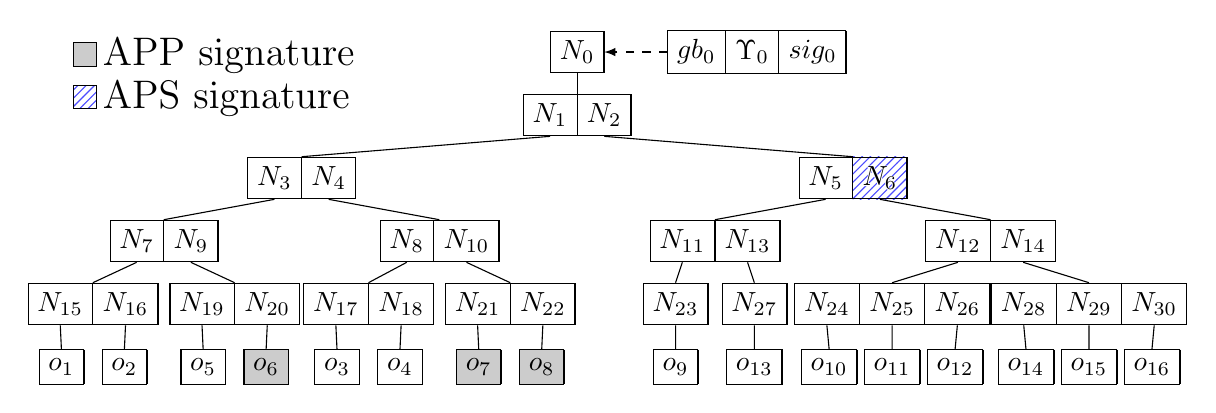
\begin{tikzpicture}
  \tikzstyle{tree node}=[
  rectangle split,
  rectangle split horizontal,
  rectangle split ignore empty parts,
  draw
  ]
  \tikzstyle{tree}=[
  every node/.style={tree node},
  edge from parent path={},
  level/.style={level distance=0.8cm},
  level 2/.style={sibling distance=7cm},
  level 3/.style={sibling distance=3.5cm},
  level 4/.style={sibling distance=1.8cm},
  level 5/.style={sibling distance=0.8cm},
  ]

  \path[tree] node (root) {$N_0$}
  child {
    node (l1) {
      \nodepart{one} $N_1$ \nodepart{two} $N_2$
    }
    child {
      node (l21) {
        \nodepart{one} $N_{3}$ \nodepart{two} $N_{4}$
      }
      child {
        node (l31) {
          \nodepart{one} $N_{7}$ \nodepart{two} $N_{9}$
        }
        child {
          node (l41) {
            \nodepart{one} $N_{15}$ \nodepart{two} $N_{16}$
          }
          child {node (o1) {$o_1$}}
          child {node (o2) {$o_2$}}
        }
        child {
          node (l42) {
            \nodepart{one} $N_{19}$ \nodepart{two} $N_{20}$
          }
          child {node (o5) {$o_5$}}
          child {node [fill=black!20, text=black] (o6) {$o_6$}}
        }
      }
      child {
        node (l32) {
          \nodepart{one} $N_{8}$ \nodepart{two} $N_{10}$
        }
        child {
          node (l43) {
            \nodepart{one} $N_{17}$ \nodepart{two} $N_{18}$
          }
          child {node (o3) {$o_3$}}
          child {node (o4) {$o_4$}}
        }
        child {
          node (l44) {
            \nodepart{one} $N_{21}$ \nodepart{two} $N_{22}$
          }
          child {node [fill=black!20, text=black] (o7) {$o_7$}}
          child {node [fill=black!20, text=black] (o8) {$o_8$}}
        }
      }
    }
    child{
      node (l22) {
        \nodepart{one} $N_{5}$ \nodepart{two} \contour{white}{$N_{6}$}
      }
      child {
        node (l33) {
          \nodepart{one} $N_{11}$ \nodepart{two} $N_{13}$
        }
        child [sibling distance=1cm] {
          node (l45) {$N_{23}$}
          child {node (o9) {$o_9$}}
        }
        child [sibling distance=1cm] {
          node (l46) {$N_{27}$}
          child {node (o13) {$o_{13}$}}
        }
      }
      child {
        node (l34) {
          \nodepart{one} $N_{12}$ \nodepart{two} $N_{14}$
        }
        child [sibling distance=2.5cm] {
          node (l47) {
            \nodepart{one} $N_{24}$
            \nodepart{two} $N_{25}$
            \nodepart{three} $N_{26}$
          }
          child {node (o10) {$o_{10}$}}
          child {node (o11) {$o_{11}$}}
          child {node (o12) {$o_{12}$}}
        }
        child [sibling distance=2.5cm] {
          node (l48) {
            \nodepart{one} $N_{28}$
            \nodepart{two} $N_{29}$
            \nodepart{three} $N_{30}$
          }
          child {node (o14) {$o_{14}$}}
          child {node (o15) {$o_{15}$}}
          child {node (o16) {$o_{16}$}}
        }
      }
    }
  };

  \begin{pgfonlayer}{background}
    \fill[pattern=north east lines,pattern color=blue!70] (l22.one split north) rectangle (l22.two split south);
  \end{pgfonlayer}

  \foreach \a/\b in {
    root.south/l1,
    l1.one south/l21,
    l1.two south/l22,
    l21.one south/l31,
    l21.two south/l32,
    l22.one south/l33,
    l22.two south/l34,
    l31.one south/l41,
    l31.two south/l42,
    l32.one south/l43,
    l32.two south/l44,
    l33.one south/l45,
    l33.two south/l46,
    l34.one south/l47,
    l34.two south/l48,
    l41.one south/o1,
    l41.two south/o2,
    l42.one south/o5,
    l42.two south/o6,
    l43.one south/o3,
    l43.two south/o4,
    l44.one south/o7,
    l44.two south/o8,
    l45.south/o9,
    l46.south/o13,
    l47.one south/o10,
    l47.two south/o11,
    l47.three south/o12,
    l48.one south/o14,
    l48.two south/o15,
    l48.three south/o16%
  }
  \draw [style=edge from parent] (\a) -- (\b.north);

  \node[tree node,right=0.8cm of root] (data)
  {$gb_0$ \nodepart{two} $\Upsilon_0$ \nodepart{three} $sig_0$};

  \draw[dashed,-latex] (data) -- (root);

  \begin{customlegend}[
    legend cell align=left,
    legend image code/.code={%
      \draw[#1] (0cm,-0.15cm) rectangle (0.3cm,0.15cm);
    },
    legend style={draw=none,left=2.3cm of root,yshift=-0.3cm,font={\Large}}
    ]
    \addlegendimage{black,fill=black!20}
    \addlegendentry{APP signature}
    \addlegendimage{black,pattern=north east lines,pattern color=blue!70}
    \addlegendentry{APS signature}
  \end{customlegend}
\end{tikzpicture}
}
          \caption{Index}
        \end{subfigure}
        \caption{Access-Policy-Preserving $k$-d-Tree (AP$^2k$d-Tree)}
      \end{figure}
  \end{itemize}
\end{frame}

\begingroup
\setbeamertemplate{frametitle continuation}{}
\begin{frame}[t,allowframebreaks]{\refname}
  \bookmark[page=\thepage,startatroot]{\refname}
  \setbeamertemplate{bibliography item}[text]
  \renewcommand*{\bibfont}{\scriptsize}
  \printbibliography[heading=none]%
\end{frame}
\endgroup

\end{document}
